\documentclass[11pt]{exam}
\RequirePackage{amssymb, amsfonts, amsmath, latexsym, verbatim, xspace, setspace}
\RequirePackage{tikz, pgflibraryplotmarks}
\usetikzlibrary{shapes.geometric,arrows,fit,matrix,positioning}
\tikzset
{
    treenode/.style = {circle, draw=black, align=center,
                          minimum size=1cm, anchor=center},
}



\usepackage[none]{hyphenat}
\usepackage[margin=1in]{geometry}
\usepackage{algorithm}
\usepackage{cancel}
\usepackage{multirow}
\usepackage{framed}
\usepackage{amsmath}
\usepackage{amsthm}
\usepackage{amssymb}
\usepackage{qtree}
\usepackage{venndiagram}
\usepackage{mathtools}
\usetikzlibrary{datavisualization}
\usetikzlibrary{datavisualization.formats.functions}
\newtheorem*{theorem*}{Theorem}
\usepackage{pgfplots}
\usepackage{ulem}
\usepackage{listings}
\usepackage{tikz}
\usepackage[noend]{algpseudocode}
\usetikzlibrary{arrows,automata,positioning}
\usetikzlibrary{arrows,positioning,shapes,fit,calc}
\usetikzlibrary{chains,fit,shapes}
\usepackage{color}   %May be necessary if you want to color links
\usepackage{hyperref}
\hypersetup{
    colorlinks=true, %set true if you want colored links
    linktoc=all,     %set to all if you want both sections and subsections linked
    linkcolor=black,  %choose some color if you want links to stand out
}

\pgfdeclarelayer{background}
\pgfsetlayers{background,main}

\usepackage{color}
\usepackage{bold-extra}

\definecolor{dkgreen}{rgb}{0,0.6,0}
\definecolor{gray}{rgb}{0.5,0.5,0.5}
\definecolor{mauve}{rgb}{0.58,0,0.82}
\lstset{
	language=python, % Replace
	basicstyle={\footnotesize\ttfamily},
	keywordstyle={\bfseries\color{blue}},
	commentstyle=\color{dkgreen},
	stringstyle={\slshape\color{mauve}},
	numberstyle=\footnotesize,
	numbers=left,
	showstringspaces=false,
	breaklines=true,
	tabsize=4,
	frame=tb
}


\newcommand\numberthis{\addtocounter{equation}{1}\tag{\theequation}}
 
\newcommand{\rowSpace}{1.2ex}
\singlespacing
 \newcommand\tab[1][1cm]{\hspace*{#1}}

\newtheorem{theorem}{Theorem}[section]
\newtheorem{lemma}[theorem]{lemma}
\begin{document} 

\vspace*{20mm}
 
\begin{center}
\Huge{CS321 Theory of Computation}\\

\vspace{10mm}

\Huge{Lecture Notes}\\

\vspace{10mm}

\large{Created by Blake Cecil}\\

\end{center}



\newpage 

\begin{center}
\huge Preface
\vspace{5mm}
\end{center}
\normalsize{
What is computation? In the age of the digital computer this question may seem irrelevant. Consider the purpose of this class to convince you otherwise. With artificial intelligence pushing the limits of what a computer can do this question has in fact become more important to consider than ever before. And while it is easy to get lost in the details of the particular machines we explore in this class it is important to remember that the brilliant people that first discovered them, did so in their desire to understand the very limits of intelligence itself.\\

In this class we will explore what it takes to build a theory capable of describing such limits. Starting with the humble finite automata, and culminating in Turing Machines. Throughout this journey one thing will remain constant, exceptionally simple rules give birth to enormous amounts of complexity. We will also find that much of the theory we develop has profound implications for practical applications. From "regex", to compilers, to programming language design and static analysis of programs. The theory of computation provides deep insights into all of these subjects.\\

At its heart the theory we develop herein is motivated by exploring the limits of human thought. In doing so we find there are, in a very real sense, things we can never know, problems we will never solve, and worlds of computation beyond our current conception. Let us begin this journey.}


\newpage 

\tableofcontents

\newpage
\section{Languages}

Naively we can thing of a language as a set of strings, a string is a sequence of characters, ex "cat", "dog".
We denote the alphabet of the language as
\begin{center}
$\Sigma = \{a,b,c, \cdots, z\}$
\end{center} 

Ex: Passwords of length five containing at least one letter and at least one digit

\begin{center}
$L = \{0000A, 0000B, A1111, AAAA2, \cdots \}$\\
$\Sigma = \{0,1, \cdots, 9, A , B , \cdots , Z \}$ 
\end{center} 

Note that we distinguish between the language and the alphabet, and that this is a finite language.

Ex: 
\begin{center}
$L = \{a^nb^n | n \geq 0 \}$\\
$L = \{ \lambda, ab, aabb, aaabbb, \cdots \}$\\
$\Sigma = \{a,b\}$\\ 
\end{center}

Notice that despite having a finite alphabet we have an infinite language, it is the construction rules that determine the complexity of the language not the alphabet.

Typically alphabets will be small and we will can use variables to work with strings, e.g  $u = aabb, v = ab$. 

\subsection{Operations}

Let $w = a_1a_2\cdots a_m, v=b_1b_2\cdots b_m$ then we define string concatenation as 
\begin{center}
$wv = a_1a_2\cdots a_mb_1b_2\cdots b_m$
\end{center}
We denote string reversal as $w^R$ and define it to be
\begin{center}
$w^R = a_m \cdots a_2a_1$
\end{center}
We denote the length of a string as $|w|$ and it can be thought of inductively as
\begin{center}
$|a| = 1$\\
$|va| = |v| + 1$\\
$\forall a \in \Sigma, v \in L$
\end{center}

Ex: 
\begin{center}
$|a| = 1$\\
$|aabb| = 4$
\end{center}


\begin{theorem}
Let $\Sigma$ be an alphabet and $L$ be a language over it. Let $u,v \in L$ then we have that $|uv| = |u| + |v|$.
\end{theorem}
\begin{proof}
 We proceed by induction. By definition the base case is trivially true. Assume that the identity holds for strings of length $n$ and let $|u| = n$ and $|v| = n+1$. Then there exists $y \in \Sigma$ and $x \in L$ such that $v = xy$. So $|v| = |x| + 1$ and $|uv| = |u| + |x| + 1$ by the induction hypothesis so $|uv| = |u| + |v|$ as desired.
\end{proof}
   

Ex:
\begin{center}
$u = aabb, v = bbb$\\
$uv = aabbbbb$\\
$|uv| = 7$
\end{center}

Finally note that $\lambda$, the "empty string", causes a wrinkle in many definitions, i.e $|\lambda| = 0$ and $\forall x \in L, \lambda x = x \lambda = x$. \\


We define a substring of a string to be any sub sequence of consecutive characters.

Ex:
\begin{center}
$a \underline{abb} a, abb$\\
$a \underline{bab} a, bab$\\
\end{center}

We simply appeal to the intuitive notion of a prefix and suffix, note that for any string the set of prefixes and suffixes always share at least two elements $\lambda$ and the whole string.

Ex:
\begin{center}
$abbab$\\
Prefix $= \{\lambda, a, ab, abb, abba, abbab \}$\\
Suffix $= \{\lambda, b, ab, bab, bbab, abbab \}$\\
\end{center}


We define exponentiation in an intuitive manner, let $w \in L$ then we have that

\begin{center}
$w^0 = \lambda$\\
$w^n = \underbrace{ww \cdots w}_\text{$n$ times}$\\
\end{center}


Another fundamental operation is $\Sigma^*$, the set of all possible strings using an alphabet $\Sigma$. This operation is of particular importance because it leads to our first formal definition of a language. Let $\Sigma$ be some alphabet, then a language $L$ is simply any subset of $\Sigma^*$. \\ 

Ex:

\begin{center}
$\Sigma = \{a,b\}$\\
$\Sigma^* =  \{\lambda, a, b, aba, ba, bbb, \cdots \}$\\

$L = \{\lambda\}$\\
$L = \{a,ba,ababa\}$\\
$L = \{\lambda, a, aa, aaa, \cdots \}$\\
\end{center}

We also have $\Sigma^+$ which is defined as $\Sigma^+ =  \Sigma^* - \{\lambda\}$.

The usual set operations also apply to languages with $\cup, \cap, -$ all behaving as usual, and the complement defined as $L^c = \Sigma^* - L$.

Ex:
\begin{center}
$\{a,b\}^c = \{\lambda,aa,ab,baba, \cdots \}$\\
\end{center}

Many of the familiar operations on strings can also be extended to languages. Much like reverse for strings we have reverse for languages which is defined as

\begin{center}
$L^R = \{ w^R | w \in L \}$\\
\end{center}

Ex:

\begin{center}
$L = \{ a^nb^n | n \geq 0 \}$\\
$L^R = \{b^na^n | n \geq 0 \}$\\
\end{center}

We can also define the concatenation of two languages as 

\begin{center}
$L_1L_2 = \{xy | x \in L_1, y \in L_2 \}$
\end{center}

Ex:

\begin{center}
$\{a,ab,ba\}\{b,aa\} = \{ab,aaa,abb,abaa,bab,baaa\}$\\
\end{center}

Using this the power of a language can be defined as
\begin{center}
$L^0 = \{\lambda\}$\\
$L^n = \underbrace{LL \cdots L}_{\text{n times}}$\\
\end{center}

Ex:

\begin{center}
$L = \{a^nb^n | n \geq 0\}$\\
$L^2 = \{a^nb^na^mb^m | n,n \geq 0 \}$\\ 
$aabbaaabbb \in L^2$\\
\end{center}

With the notion of powers defined we can now introduce another important operation commonly known as the "Kleene star"

\begin{center}
$L^* = L^0 \cup L^1 \cup L^2 \cup \cdots$\\
We also have the positive variant
\begin{align*}
L^+ &= L^1 \cup L^2 \cup \cdots\\
	&= L^* - \{\lambda\}\\
\end{align*}
\end{center}

\newpage

\section{Finite Automata}

In this section we explore two fundamental types of automata, deterministic and non deterministic finite automata (DFA, NFA) respectively. We restrict our focus to so called "accepters" which either accept or reject input.



\subsection{Deterministic Finite Automata}
Formally we define a DFA $M$ as the following quintuple

\begin{center}
$M = (Q,\Sigma,\delta,q_0,F)$\\
$Q$ : Set of states\\
$\Sigma$ : Alphabet\\
$\delta$ : Transition function\\
$q_0$ : initial state\\
$F$ : Set of final states\\
\end{center}

In DFA's we require $\delta$ to be a total function in other words $\delta : Q \times \Sigma \rightarrow Q$. In order to work in a more intuitive manner we can extend $\delta$ to process strings rather than single characters.\\

Formally we define this extended function $\delta^*$ to be

\begin{center}
Let $\sigma \in \Sigma$ and $w \in \Sigma^+$\\
$\delta^*(q,\lambda) = q$\\
$\delta^*(q,w\sigma) = \delta(\delta^*(q,w),\sigma)$\\
\end{center}

This recursive definition is tedious to use and is defined merely to ensure that our intuitions of processing strings can be made rigorous.\\

To connect languages with DFA's we introduce the following notion that allows us to rigorously define what it means for a DFA to accept or recognize a language. Let $M$ be a DFA then we define the language accepted by $M$ and its complement as 

\begin{center}
$L(M) = \{ x \in \Sigma^* | \delta^*(q_0,x) \in F \}$\\
$L^c(M) = \{ x \in \Sigma^* | \delta^*(q_0,x) \notin F \}$\\
\end{center}

We can now define a fundamental notion, regularity of a language. Let $L$ be a language, then we call $L$ regular if $\exists \text{ DFA } M$ such that $L = L(M)$. Because there are languages that are not regular this notion will be a useful tool in exploring the complexity of languages and the power of the machines that accept them.

\subsection{Non Deterministic Finite Automata}



Nondeterministic Finite automata are another flavor that have the following peculiar property, \emph{if there is any walk to any final state, they will find it}. This is reflected in the fact that we do not require every state to have a transition for ever character in the alphabet. We also allow $\lambda$ transitions which allow a change of state without actually consuming any characters in the input.\\

\newpage 
Formally we define an NFA as
\begin{center}
$M = (Q,\Sigma,\delta,q_0,F)$\\
$Q$ : Set of states\\
$\Sigma$ : Alphabet\\
$\delta$ : Transition function\\
$q_0$ : initial state\\
$F$ : Set of final states\\
\end{center}
With the very important change to the transition function $\delta : Q \times (\Sigma \cup \{\lambda\}) \rightarrow 2^Q$.
We can still define $\delta^*$ in the same manner but we must make the following slight change to the notion of a language accepted by an NFA.\\

Let $N$ be an NFA then we define the language accepted by $N$ as 
\begin{center}
$L(N) = \{w \in \Sigma^* | \delta^*(q_0, w) \cap F \neq \emptyset \}$
\end{center}

\subsection{NFA = DFA, The Rabin–Scott powerset construction}
Rather surprisingly NFA's are in some sense nothing more than a convenience of notation, any language recognized by an NFA can also be recognized in a DFA as we will prove shortly.\\

In order to analyze the power of automata we first introduce the notion of equivalence. Let $M_1,M_2$ Be automata, then we say $M_1$ and $M_2$ are equivalent if $L(M_1) = L(M_2)$\\

We can now prove that DFA's and NFA's have the same power.


\begin{theorem}
Let $NFA = \{\text{ Languages accepted by NFA's } \}$ and $DFA = \{ \text{ Languages accepted by DFA's } \}$, then $NFA = DFA$\\
\end{theorem}

\begin{proof}
Let $L \in DFA$ then we trivially have that every DFA is an NFA so $L \in NFA$ and $DFA \subseteq NFA$.  Now let $L' \in NFA$. We first describe an algorithm that allows us to convert any NFA to a DFA, which will in turn allows us to prove that $L' \in DFA$. Consider the following algorithm

\newpage 

\begin{enumerate}
\item Let the initial state of the NFA be $q_0$, then create an initial state for the DFA and label it $\{q_0\}$.

\item Now fix $a \in \Sigma$ and create a label for every DFA state and $\forall q_i \in Q$ compute $\bigcup \delta^*(q_i,a)$  and label this as the new state in the DFA and add it to the transition function of the DFA.

\item Repeat step 2 for all letters in $\Sigma$ until no more transitions can be added

\item For any DFA state with label $\{q_i,q_j, \dots , q_m\}$ if any of the $q$'s are final states in the NFA make $\{q_i,q_j, \dots , q_m\}$ a final state.
\end{enumerate}

Ex:\\
Consider transforming the following NFA:\\
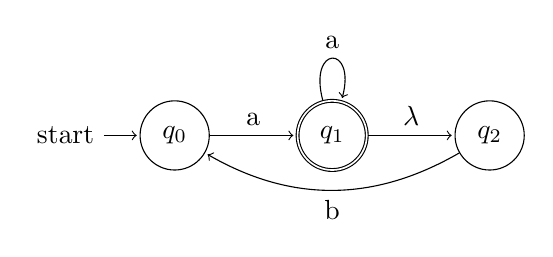
\begin{tikzpicture}[shorten >=1pt,node distance=2cm,on grid,auto] 
   \node[state,initial] (q_0)   {$q_0$}; 
   \node[state,accepting] (q_1) [right=of q_0] {$q_1$}; 
   \node[state] (q_2) [right=of q_1] {$q_2$}; 
    \path[->] 
    (q_0) edge  node {a} (q_1)
    (q_1) edge  node  {$\lambda$} (q_2)
          edge [loop above] node {a} ()
    (q_2) edge [bend left, below] node {b} (q_0);
\end{tikzpicture}

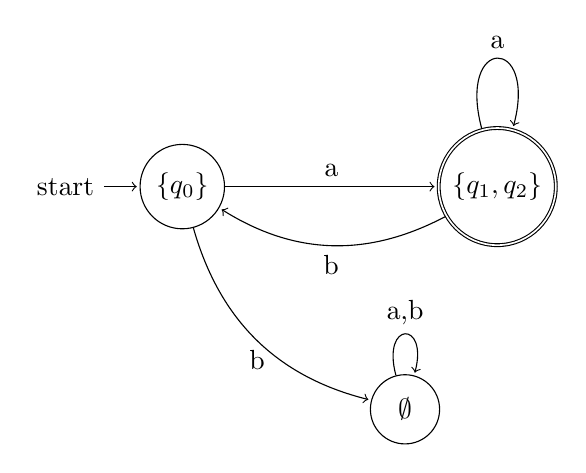
\begin{tikzpicture}[shorten >=1pt,node distance=4cm,on grid,auto] 
   \node[state,initial] (q_0)   {\{$q_0$\}}; 
   \node[state,accepting] (q_1) [right=of q_0] {$\{q_1,q_2\}$}; 
   \node[state] (q_2) [below right=of q_0] {$\emptyset$}; 
    \path[->] 
    (q_0) edge  node {a} (q_1)
          edge [bend right, below] node {b} (q_2)
    (q_1) edge [bend left, below] node  {b} (q_0)
          edge [loop above] node {a} ()
    (q_2) edge [loop above] node {a,b} ();
\end{tikzpicture}\\


  
Using this construction we can now prove that our DFA is equivalent to the NFA we constructed it from which will in turn allow us to conclude that $L' \in DFA$.\\

Let $M$ be some $NFA$ and construct $M'$ using the algorithm described. Now consider $L(M)$ and $L(M')$. We will show that $L(M) \subseteq L(M')$ and omit the details of the other inclusion since it is nearly identical.\\

 Let $w \in L(M)$ then we will show there exists a walk in the DFA and thereby that $w \in L(M')$. We proceed by induction on the length of $w$. To prove the base case let $w = a_1$ and suppose that $\delta(a_1) = q$ for some $q$ in the final states of the NFA. Then by construction of the algorithm we have that $\delta(q_0,a)$ is a final state in the DFA so the base case holds.\\
 
  Now suppose that the inductive hypothesis holds for all  $w \in L(M)$ such that $1 \leq |w| \leq k$ and that we have $w \in L(M)$ such that $|w| = k + 1$, now consider that $w$ can be broken up into $a \in \Sigma$ and $y \in \Sigma*$ such that  $w = ya$ and we can apply the inductive hypothesis to $y$ and $a$ which implies that the theorem holds for $k + 1$ so we have that $\forall w \in L(M)$ there exists an equivalent walk in our DFA. \\

This allows us to conclude that $L(M) \subseteq L(M')$, a similar argument allows us to show that $L(M') \subseteq L(M)$ which in turn implies $L(M) = L(M')$, finally yielding that $DFA = NFA$ as desired. 

\end{proof}

\newpage

\section{Regular Expressions}

In our exploration of understanding the regular languages we will uncover the connection between so called "regular expressions" and the regular languages. Regular expressions find much practical use and often go by the name "regex" for short. We will see their connection to regular languages and see how they often provide a succinct and easy way to describe a language.\\

Let $r$ be a regular expression, then we can define $L(r)$, the language recognized by $r$ in the following recursive manner


\begin{center}
$L(\emptyset) = \emptyset$\\
$L(\lambda) = \lambda$\\
$L(a) = \{a\} \ \forall a \in \Sigma$\\
Let $r_1, r_2$ be regular expressions then\\
$L(r_1 + r_2) = L(r_1) \cup L(r_2)$\\
$L(r_1 \dot r_2) = L(r_1)L(r_2)$\\
$L(r_1^*) = (L(r_1))^*$\\
$L((r_1)) = L(r_1)$\\
\end{center}

Ex:

\begin{center}
$r = (a + b) \dot a^*$\\
\begin{align*}
L((a + b) \dot a^*) &= L((a+b))L(a^*)\\
&= (L(a) \cup L(b))L(a)^*\\
&= \{a,b\}\{\lambda,a,aa,aaa,\dots\}\\
&= \{a,aa,aaa,\dots,b,ba,baa,baaa,\dots\}\\ 
\end{align*}
\end{center}

Ex:
\begin{center}
$r = (aa)^*(bb)^*b$\\
$L(r) = \{a^{2n}b^{2m}b | n,m \geq 0 \}$
\end{center}

Ex:
\begin{center}
$r = (0+1)^*00(0+1)^*$\\
$L(r) = \{ \text{ all strings with at least two consective 0's } \}$
\end{center}

Ex: 
\begin{center}
$\Sigma = \{0,1\}$
All strings $w \in \Sigma^*$ such that $|w| \text{ mod } 3 = 0$\\

$r = ((0+1)(0+1)(0+1))^*$\\
\end{center}

\subsection{Regular Expressions = NFA, Thompsons Construction and Kleenes Algorithm}
We can now proceed to the central result of the study of regular expressions; all languages generated by them are regular.

\begin{theorem}
Let $Regex = \{ \text{ Languages generated by regular expressions } \}, R = \{ \text{ regular languages } \}$. Then $Regex = R$
\end{theorem}
\begin{proof}
We first prove that $Regex \subset R$. Let $r \ Regex$, then we proceed by induction on the number of operations in $r$. For the base case we can handle $\emptyset, \lambda$ and the single character with the following simple automata

\begin{center}
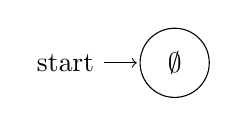
\begin{tikzpicture}[shorten >=1pt,node distance=4cm,on grid,auto] 
   \node[state,initial] (q_0)   {$\emptyset$}; 
\end{tikzpicture}

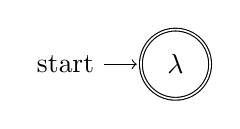
\begin{tikzpicture}[shorten >=1pt,node distance=4cm,on grid,auto] 
   \node[state,initial,accepting] (q_0)   {$\lambda$}; 
\end{tikzpicture}

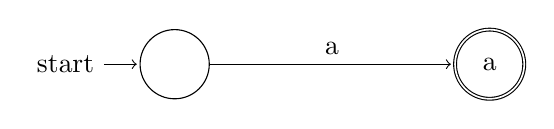
\begin{tikzpicture}[shorten >=1pt,node distance=4cm,on grid,auto] 
   \node[state,initial] (q_0)   {}; 
   \node[state,accepting] (q_1) [right=of q_0] {a};  
    \path[->] 
    (q_0) edge  node {a} (q_1);
\end{tikzpicture}
\end{center}

With the base case established we can proceed with the argument. Assume that for all regular expressions of $n$ operators have a resulting NFA. Then let $r_1,r_2$ be two regular with  expressions $n$ and 1 operators respectively then we simply need to prove that for each operator $+,\dot,*$ we can construct an NFA that recognizes the new language.\\

By the induction hypothesis we have to NFA's $M_1,M_2$ such that $M_1(r_1),M_2(r_2)$ are regular.

Then for $L(r_1 + r_2)$ we can construct the following NFA

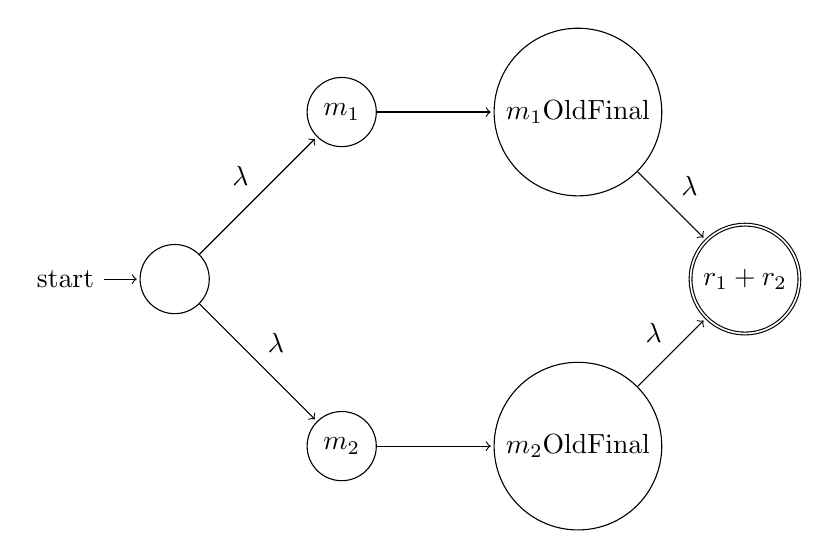
\begin{tikzpicture}[shorten >=1pt,node distance=3cm,on grid,auto] 
   \node[state,initial] (q_0)   {}; 
   \node[state] (m_1) [above right=of q_0] {$m_1$}; 
   \node [state] (m_2) [below right= of q_0] {$m_2$};
   \node [state] (m_1f) [right= of m_1] {$m_1$OldFinal};
   \node [state] (m_2f) [right= of m_2] {$m_2$OldFinal}; 
   \node [state,accepting] (final) [above right= of m_2f] {$r_1 + r_2$};
    \path[->] 
    (q_0) edge  node {$\lambda$} (m_1)
    (q_0) edge  node {$\lambda$} (m_2)
    (m_1) edge node {} (m_1f)
    (m_2) edge node {} (m_2f)
    (m_1f) edge node {$\lambda$} (final)
    (m_2f) edge node {$\lambda$} (final);
\end{tikzpicture}

For $L(r_1r_2)$ we can construct the product NFA

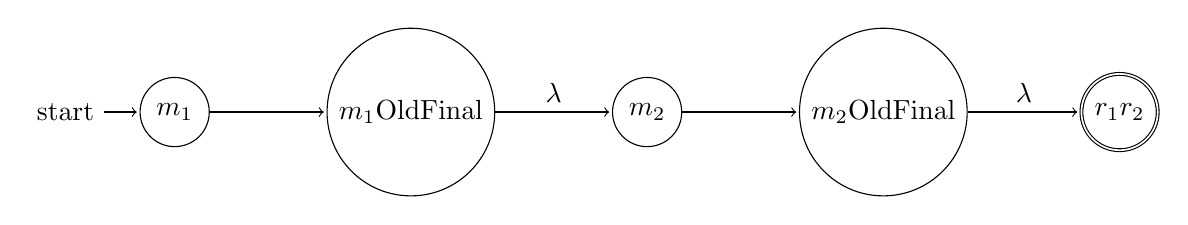
\begin{tikzpicture}[shorten >=1pt,node distance=3cm,on grid,auto]  
   \node[state,initial] (m_1)  {$m_1$};
   \node [state] (m_1f) [right= of m_1] {$m_1$OldFinal}; 
   \node [state] (m_2) [right= of m_1f] {$m_2$};
   \node [state] (m_2f) [right= of m_2] {$m_2$OldFinal}; 
   \node [state,accepting] (final) [right= of m_2f] {$r_1r_2$};
    \path[->] 
    (m_1) edge  node {} (m_1f)
    (m_1f) edge  node {$\lambda$} (m_2)
    (m_2) edge node {} (m_2f)
    (m_2f) edge node {$\lambda$} (final);
\end{tikzpicture}

\newpage

And Finally we have the star closure represented by the following NFA

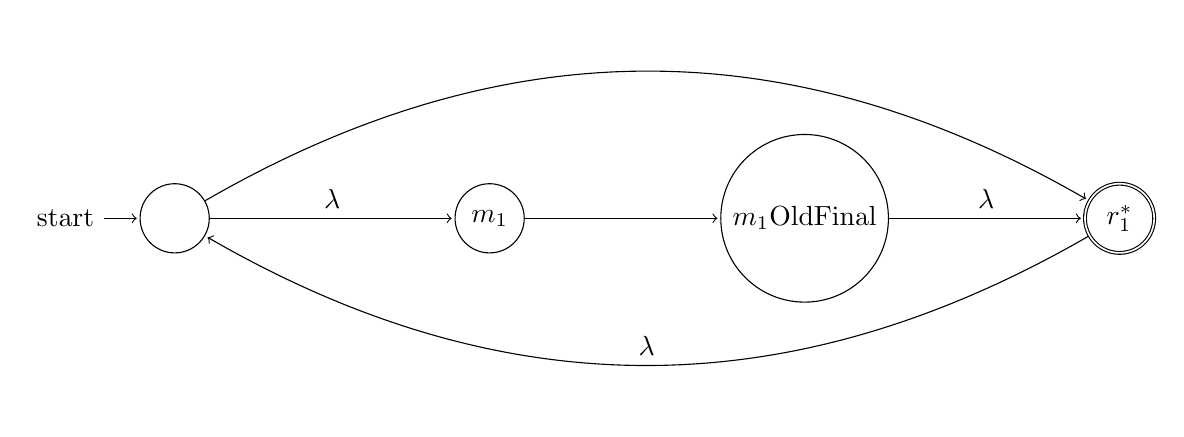
\begin{tikzpicture}[shorten >=1pt,node distance=4cm,on grid,auto]  
   \node [state,initial] (q_0)  {};
   \node [state] (m_1) [right= of q_0] {$m_1$};
   \node [state] (m_1f) [right= of m_1] {$m_1$OldFinal}; 
   \node [state,accepting] (final) [right= of m_1f] {$r_1^*$};
    \path[->] 
    (q_0) edge  node {$\lambda$} (m_1)
    	  edge  [bend left, above] node {} (final)
    (m_1) edge node {} (m_1f)
    (m_1f) edge node {$\lambda$} (final)
    (final) edge  [bend left, above] node  {$\lambda$} (q_0);  
\end{tikzpicture}

And trivially $(r_1)$ or $(r_2)$ is a regular language. So we have that $r \in R$ which implies $Regex \subseteq R$.\\

Now let $l \in R$ then there exists an NFA $M$ such that $L(M) = l$. We will then construct a regular expression from $M$. First we consider a generalized transition graph where edges can have regular expressions rather than just characters from the alphabet. For an intuition of such a construction consider the following

\begin{center}
\begin{tikzpicture}[shorten >=1pt,node distance=4cm,on grid,auto]  
   \node [state,initial] (q_0)  {};
   \node [state] (q_1) [right= of q_0] {$q_1$};
   \node [state, accepting] (q_2) [right= of m_1] {$q_2$}; 
    \path[->] 
    (q_0) edge  [bend right, below] node {b} (q_1)
    (q_1) edge node {a,b} (q_2)
          edge [bend right, above] node {a} (q_0)
          edge [loop, above] node {b} ()
    (q_2) edge [loop, above] node {b} ();  
\end{tikzpicture}
\begin{tikzpicture}[shorten >=1pt,node distance=4cm,on grid,auto]  
   \node [state,initial] (q_0)  {};
   \node [state] (q_1) [right= of q_0] {$q_1$};
   \node [state, accepting] (q_2) [right= of m_1] {$q_2$}; 
    \path[->] 
    (q_0) edge  [bend right, below] node {b} (q_1)
    (q_1) edge node {a+b} (q_2)
          edge [bend right, above] node {a} (q_0)
          edge [loop, above] node {b} ()
    (q_2) edge [loop, above] node {b} ();  
\end{tikzpicture}
\begin{tikzpicture}[shorten >=1pt,node distance=4cm,on grid,auto]  
   \node [state,initial] (q_0)  {};
   \node [state] (q_1) [right= of q_0] {$q_1$};
   \node [state, accepting] (q_2) [right= of m_1] {$q_2$}; 
    \path[->] 
    (q_0) edge  [bend right, below] node {b} (q_1)
    (q_1) edge node {a,b} (q_2)
          edge [bend right, above] node {a} (q_0)
          edge [loop, above] node {b} ()
    (q_2) edge [loop, above] node {b} ();  
\end{tikzpicture}
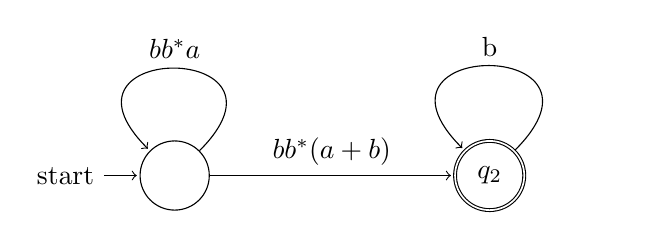
\begin{tikzpicture}[shorten >=1pt,node distance=4cm,on grid,auto]  
   \node [state,initial] (q_0)  {};
   \node [state, accepting] (q_2) [right= of q_0] {$q_2$}; 
    \path[->] 
    (q_0) edge node {$bb^*(a+b)$} (q_2)
          edge [loop, above] node {$bb^*a$} (q_0)
    (q_2) edge [loop, above] node {b} ();  
\end{tikzpicture}

Which gives us the final regular expression $(bb^*a)^*bb^*(a+b)b^*$
\end{center}

The beauty of this construction is that we really only need to know how to decompose 3 nodes and then we can let induction do the rest. So in general consider that 

\begin{center}
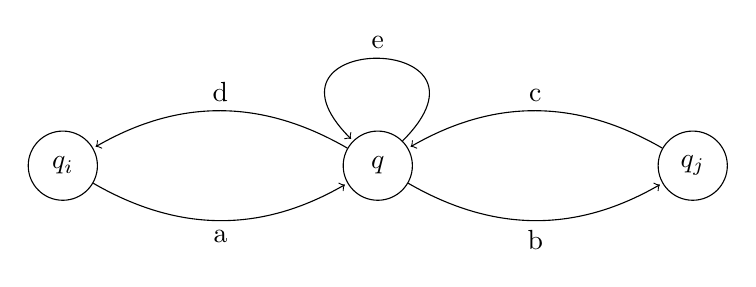
\begin{tikzpicture}[shorten >=1pt,node distance=4cm,on grid,auto]  
   \node [state] (q_i)  {$q_i$};
   \node [state] (q) [right= of q_i] {$q$};
   \node [state] (q_j) [right= of q] {$q_j$}; 
    \path[->] 
    (q_i) edge  [bend right, below] node {a} (q)
    (q) edge [loop, above] node {e} ()
        edge [bend right, below] node {b} (q_j)
    	edge [bend right, above] node {d} (q_i)
    (q_j) edge [bend right, above] node {c} (q);  
\end{tikzpicture}
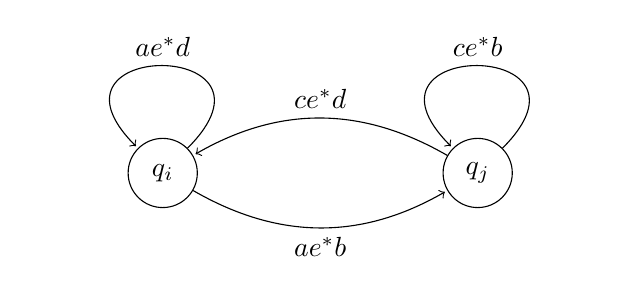
\begin{tikzpicture}[shorten >=1pt,node distance=4cm,on grid,auto]  
   \node [state] (q_i)  {$q_i$};
   \node [state] (q_j) [right= of q_i] {$q_j$}; 
    \path[->] 
    (q_i) edge  [loop, above] node {$ae^*d$} ()
          edge  [bend right, below] node {$ae^*b$} (q_j)
    (q_j) edge [loop, above] node {$ce^*b$} ()
          edge [bend right, above] node {$ce^*d$} (q_i);  
\end{tikzpicture}

We can apply this process inductively till we have the final transition graph

\begin{tikzpicture}[shorten >=1pt,node distance=4cm,on grid,auto]  
   \node [state,initial] (q_0)  {$q_0$};
   \node [state,accepting] (q_f) [right= of q_0] {$q_f$}; 
    \path[->] 
    (q_i) edge  [loop, above] node {$r_1$} ()
          edge  [bend right, below] node {$r_2$} (q_j)
    (q_j) edge [loop, above] node {$r_4$} ()
          edge [bend right, above] node {$r_3$} (q_i);  
\end{tikzpicture}

From which we can derive our final regular expression
$r_1^*r_2(r_4 + r_3r_1^*r_2)^*$.

So for any regular language we can construct an equivalent regular expression which implies that $l \in Regex \implies R \subseteq Regex$ and we have that $Regex = R$ as desired.
\end{center}

\end{proof}

\newpage

\section{Grammars}

Grammars are a fundamental tool in not only the theory of computation but, linguistics, natural language processing, and compiler design as well. This is in part because, as we will see, grammars are actually more powerful than anything we have studied thus far. Their deeply recursive power lets us go beyond regular languages. But first we will study some restricted types of grammars and analyze their connection with regular languages.\\

Formally we define a grammar $G$ as the following 

\begin{center}
$G = (V,T,S,P)$\\
$V:$ Set of variables\\
$T:$ Set of terminal symbols\\
$S:$ Start variable\\
$P:$ Set of Production rules\\
\end{center}
 

Ex:

\begin{align*}
G &: S \rightarrow aSb\\
  &:   S \rightarrow \lambda\\
G &= (\{S\}, \{a,b\}, S, \{S \rightarrow aSb, S \rightarrow \lambda\} 
\end{align*}

We can "derive" as strings and denote this by $w_1 \stackrel{*}\implies w_n$ which is shorthand for $w_1 \implies w_2 \implies \dots \implies w_n$. With this we can then define the language of a grammar.

\begin{center}
Let $G$ be a grammar and $S$ its start variable then\\
$L(G) = \{w | S \stackrel{*}\implies w\}$\\
Is called its language
\end{center}

As previously mentioned we will first explore simple grammars, so called left-linear and right-linear grammars.\\

A right-linear grammar is one where all productions have the form $A \rightarrow  xB$ or $A \rightarrow x$ for some $x \in T^*$. A left linear grammar is the same but with productions of the form $A \rightarrow Bx$. Because most of us read left to right we will typically work with right-linear grammars in this course.\\

We call a grammar a regular grammar if it is right or left linear.

Ex:
\begin{center}
All strings of 0's and 1's that start with a 0 and end with a 1\\
$S \rightarrow 0A$\\
$A \rightarrow 0A | 1A | 1$\\
\end{center}

Ex:
\begin{center}
$L(r) = \{a^{2n}b^{2m}b | n,m \geq 0 \}$\\
$S \rightarrow aaS | bbS | b$
\end{center} 

\subsection{Grammars = NFA}
As one might expect regular grammars actually generate regular languages.

\begin{theorem}
Let $RG = \{ \text{Languages generated by regular grammars} \}, R = \{ \text{Regular languages} \}$ then $RG = R$
\end{theorem}

\begin{proof}
Let $g \ in RG$ then we will construct an NFA $M$ such that $L(g) = L(M)$
by the following algorithm. $g$ has variables $V_0,V_1,\dots$ and productions $V_i \rightarrow a_1a_2\dots a_mV_j$ or $V_i \rightarrow a_1a_2\dots a_m$. Then we construct an NFA such that each $V_i$ corresponds to a node and add a final state node $V_F$. 

\begin{center}
\begin{tikzpicture}[shorten >=1pt,node distance=4cm,on grid,auto]  
   \node [state,initial] (V_0)  {$v_0$};
   \node [state] (V_1) [above right= of V_0] {$V_1$};
   \node [state] (V_2) [below right= of V_0] {$V_2$};
   \node [state] (V_3) [right= of V_1] {$V_3$};
   \node [state] (V_4) [right= of V_2] {$V_4$};
   \node [state,accepting] (V_F) [below right= of V_3] {$V_F$};
\end{tikzpicture}
\end{center}


For each production of the form $V_i \rightarrow a_1a_2\dots a_mV_j$ we add transitions and intermediate nodes for the characters up to node $V_j$ and for any production containing only literals we do the same but connect to $V_F$.

\begin{center}
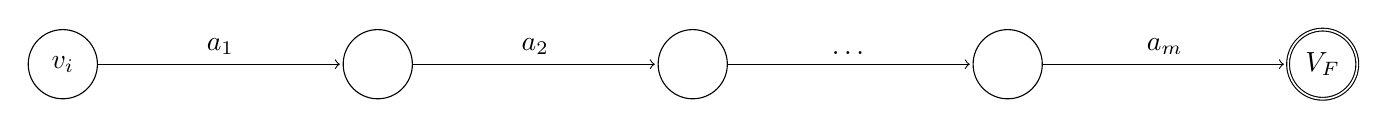
\begin{tikzpicture}[shorten >=1pt,node distance=4cm,on grid,auto]  
   \node [state] (V_i)  {$v_i$};
   \node [state] (V_1) [right= of V_i] {};
   \node [state] (V_2) [right= of V_1] {};
   \node [state] (V_3) [right= of V_2] {};
   \node [state,accepting] (V_F) [right= of V_3] {$V_F$};
   \path[->]
    (V_i) edge node {$a_1$} (V_1)
    (V_1) edge node {$a_2$} (V_2)
    (V_2) edge node {$\dots$} (V_3)
    (V_3) edge node {$a_m$} (V_F);
\end{tikzpicture}
\end{center}

So we have a resulting NFA that looks like
\begin{center}
\begin{tikzpicture}[shorten >=1pt,node distance=3cm,on grid,auto]  
   \node [state,initial] (V_0)  {$V_0$};
   \node [state] (V_1) [above right= of V_0] {$V_1$};
    \node [state] (V_6) [below right= of V_1] {};
   \node [state] (V_2) [below right= of V_0] {$V_2$};
   \node [state] (V_5) [right= of V_1] {};
   \node [state] (V_3) [right= of V_5] {$V_3$};
   \node [state] (V_7) [below right= of V_6] {};
   \node [state] (V_4) [below right= of V_7] {$V_4$};
   \node [state,accepting] (V_F) [below right= of V_3] {$V_F$};
   \path[->]
   (V_0) edge node {$a_1$} (V_1)
   (V_0) edge node {$a_3$} (V_2)
   (V_1) edge node {$a_2$} (V_5)
   (V_1) edge node {$a_3$} (V_6)
   (V_2) edge node {$a_5$} (V_4)
   (V_3) edge node {$a_5$} (V_F)
   (V_4) edge node {$a_9$} (V_F)
   (V_7) edge node {$a_8$} (V_4)
   (V_6) edge node {$a_4$} (V_7)
   (V_3) edge [bend right, above] node {$a_9$} (V_1)
   (V_5) edge node {$a_4$} (V_3);
\end{tikzpicture}
\end{center}
That corresponds to the grammar 
\begin{align*}
V_0 &\rightarrow a_1V_1 | a_3V_2\\
V_1 &\rightarrow a_2a_4V_3 | a_3a_4a_8V_4\\
V_2 &\rightarrow a_5V_4\\
V_3 &\rightarrow a_9V_1 | a_5\\
V_4 &\rightarrow a_9\\
\end{align*}
 Then we have that $L(G) = L(M)$ and $g \in R$ so $RG \subseteq R$.\\

Now let $l \in R$ then we will construct a linear grammar $G$ from the NFA M that recognizes $l$. This simply requires  that for any transition\\

\begin{center}
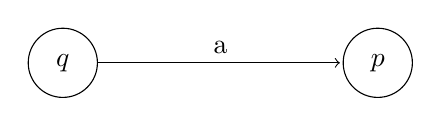
\begin{tikzpicture}[shorten >=1pt,node distance=4cm,on grid,auto]  
   \node [state] (q)  {$q$};
   \node [state] (p) [right= of q] {$p$}; 
    \path[->] 
    (q) edge  node {a} (p); 
\end{tikzpicture}
\end{center}


We add the production $q \rightarrow ap$ and for any final state we add the production $q_f \rightarrow \lambda$. Then we have that $L(G) = L(M) = l$ so $l \in RG$ which implies that $RG = R$ as desired.
\end{proof}

\newpage

\section{Closure Properties of Regular Languages}

In our desire to classify the regular languages it is very useful to study what operations the are preserved under. In other words given regular languages $L_1,L_2$ what operations e.g $\cup,\cap,*$ etc preserve the regularity of the language.\\

As it turns out regular languages are very well behaved in the sense that they are "closed" under many operations as we will prove in this section.\\

Let $L_1,L_2$ be regular languages and $l_1OldFinal,l_2OldFinal$ be their final states $l_1,l_2$ be their initial states.

\subsection{Union}
\begin{theorem}
$L_1 \cup L_2$ is a regular language
\end{theorem} 
\begin{proof}
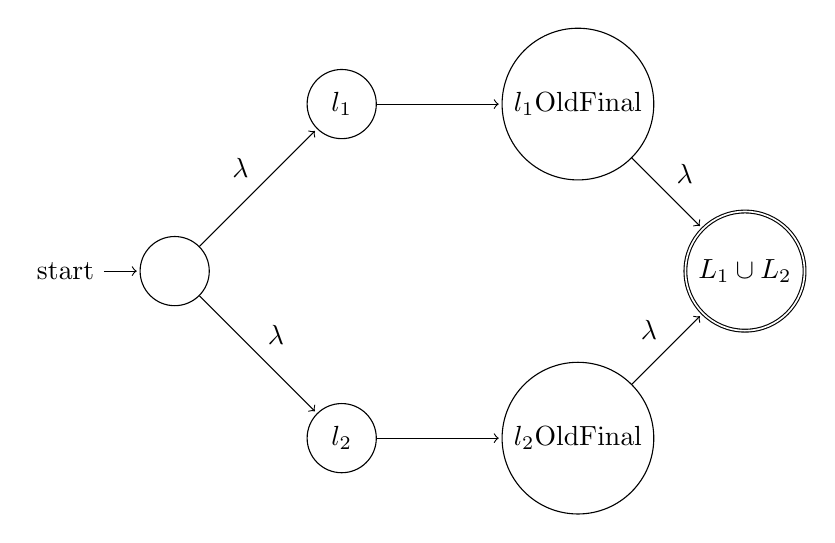
\begin{tikzpicture}[shorten >=1pt,node distance=3cm,on grid,auto] 
   \node[state,initial] (q_0)   {}; 
   \node[state] (m_1) [above right=of q_0] {$l_1$}; 
   \node [state] (m_2) [below right= of q_0] {$l_2$};
   \node [state] (m_1f) [right= of m_1] {$l_1$OldFinal};
   \node [state] (m_2f) [right= of m_2] {$l_2$OldFinal}; 
   \node [state,accepting] (final) [above right= of m_2f] {$L_1 \cup L_2$};
    \path[->] 
    (q_0) edge  node {$\lambda$} (m_1)
    (q_0) edge  node {$\lambda$} (m_2)
    (m_1) edge node {} (m_1f)
    (m_2) edge node {} (m_2f)
    (m_1f) edge node {$\lambda$} (final)
    (m_2f) edge node {$\lambda$} (final);
\end{tikzpicture}

which proves closure under union.
\end{proof}


\subsection{Concatenation}
\begin{theorem}
$L_1L_2$ is a regular language
\end{theorem}

\begin{proof}
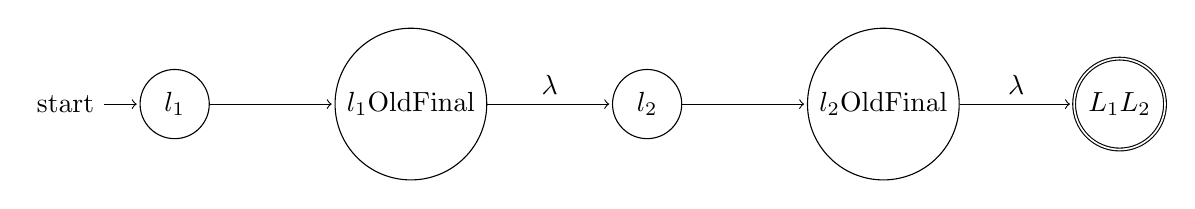
\begin{tikzpicture}[shorten >=1pt,node distance=3cm,on grid,auto]  
   \node[state,initial] (m_1)  {$l_1$};
   \node [state] (m_1f) [right= of m_1] {$l_1$OldFinal}; 
   \node [state] (m_2) [right= of m_1f] {$l_2$};
   \node [state] (m_2f) [right= of m_2] {$l_2$OldFinal}; 
   \node [state,accepting] (final) [right= of m_2f] {$L_1L_2$};
    \path[->] 
    (m_1) edge  node {} (m_1f)
    (m_1f) edge  node {$\lambda$} (m_2)
    (m_2) edge node {} (m_2f)
    (m_2f) edge node {$\lambda$} (final);
\end{tikzpicture}

which proves closure under concatenation.
\end{proof}



\subsection{Star Closure}

\begin{theorem}
$L^*$ is a regular langauge
\end{theorem}

\begin{proof}
\begin{tikzpicture}[shorten >=1pt,node distance=4cm,on grid,auto]  
   \node [state,initial] (q_0)  {};
   \node [state] (m_1) [right= of q_0] {$l_1$};
   \node [state] (m_1f) [right= of m_1] {$l_1$OldFinal}; 
   \node [state,accepting] (final) [right= of m_1f] {$L_1^*$};
    \path[->] 
    (q_0) edge  node {$\lambda$} (m_1)
    	  edge  [bend left, above] node {} (final)
    (m_1) edge node {} (m_1f)
    (m_1f) edge node {$\lambda$} (final)
    (final) edge  [bend left, above] node  {$\lambda$} (q_0);  
\end{tikzpicture}

which proves closure under the star closure operation.
\end{proof}



\subsection{Complement}
This construction is somewhat different in that we require a DFA, a trivial restriction as we can always translate a NFA into a DFA. Once this is done let $l_1$Final be the final state and $l_1Init$ be the initial. Then the complement is recognized by the following DFA

\begin{theorem}
$\overline{L} is a regular language$
\end{theorem}
\begin{proof}
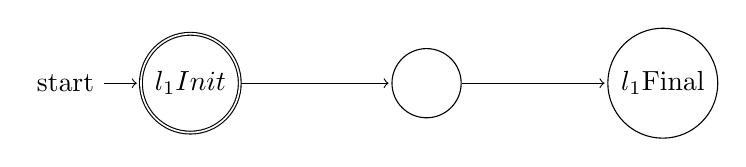
\begin{tikzpicture}[shorten >=1pt,node distance=3cm,on grid,auto]  
   \node[state,initial,accepting] (m_1)  {$l_1Init$};
   \node [state] (i) [right= of m_1] {};
   \node [state] (m_1f) [right= of i] {$l_1$Final}; 
    \path[->] 
    (m_1) edge  node {} (i)
    (i) edge  node {} (m_1f);
\end{tikzpicture}

In general we make every final state a non final state and every non final state a final state.
\end{proof}


\subsection{Product DFA}

We take brief but very useful detour to examine the "product" DFA which one can think of as the extension of the Cartesian product to DFA's. Consider the following two DFA's\\

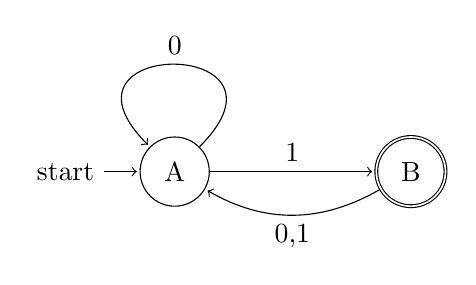
\begin{tikzpicture}[shorten >=1pt,node distance=3cm,on grid,auto]  
   \node[state,initial] (A)  {A};
   \node [state,accepting] (B) [right= of A] {B};
 
    \path[->] 
    (A) edge [loop, above] node {0} ()
        edge node {1} (B)
    (B) edge [bend left, below]  node {0,1} (A);
\end{tikzpicture}
\begin{tikzpicture}[shorten >=1pt,node distance=3cm,on grid,auto]  
   \node[state,initial,accepting] (C)  {A};
   \node [state] (D) [right= of C] {D};
 
    \path[->] 
    (A) edge [loop, above] node {1} ()
        edge node {0} (B)
    (B) edge [bend left, below]  node {1} (A)
        edge [loop, above] node {0} ();
\end{tikzpicture}\\

Then we can construct the product DFA\\
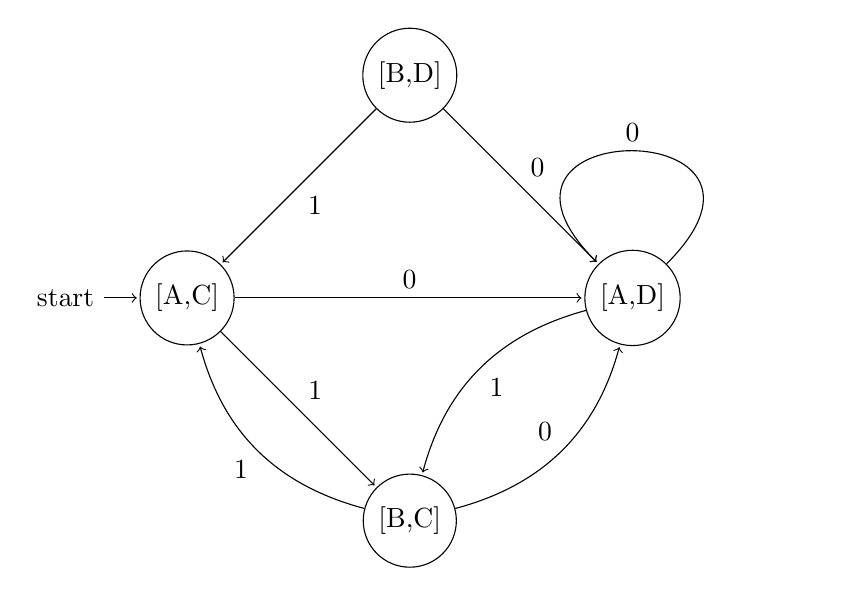
\begin{tikzpicture}[shorten >=1pt,node distance=4cm,on grid,auto]  
   \node[state,initial] (AC)  {[A,C]};

   \node [state] (BD) [above right= of AC] {[B,D]};
      \node [state] (AD) [below right= of BD] {[A,D]};
   \node [state] (BC) [below right= of AC] {[B,C]};
    \path[->] 
    (AC) edge node {1} (BC)
         edge node {0} (AD)
    (BC) edge [bend right] node {0} (AD)
         edge [bend left] node {1} (AC)
    (AD) edge [loop, above] node {0} ()
         edge [bend right] node {1} (BC)
    (BD) edge node {0} (AD)
         edge node {1} (AC);
\end{tikzpicture}\\

using this construction we can prove several closures just by choosing the final state appropriately
\subsection{Intersection}

Somewhat surprisingly the intersection of two regular languages is always regular. Using DeMorgans law we can prove this before explicitly constructing the DFA.\\

\begin{theorem}
$L_1 \cap L_2$ is a regular language
\end{theorem}
\begin{proof}
Consider that $\overline{L_1} \cup \overline{L_2}$ is regular by the previous theorems and its closure is too which implies $\overline{\overline{L_1} \cup \overline{L_2}} = L_1 \cap L_2$ is regular as well.\\
\end{proof} 

With the product DFA we can also trivially construct the intersection by making the state labeled with both final states a final state.

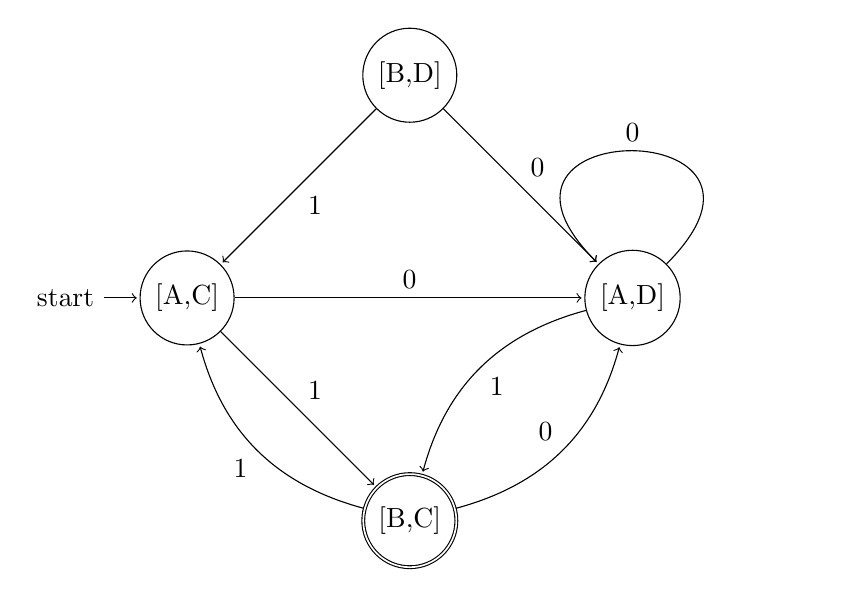
\begin{tikzpicture}[shorten >=1pt,node distance=4cm,on grid,auto]  
   \node[state,initial] (AC)  {[A,C]};

   \node [state] (BD) [above right= of AC] {[B,D]};
      \node [state] (AD) [below right= of BD] {[A,D]};
   \node [state,accepting] (BC) [below right= of AC] {[B,C]};
    \path[->] 
    (AC) edge node {1} (BC)
         edge node {0} (AD)
    (BC) edge [bend right] node {0} (AD)
         edge [bend left] node {1} (AC)
    (AD) edge [loop, above] node {0} ()
         edge [bend right] node {1} (BC)
    (BD) edge node {0} (AD)
         edge node {1} (AC);
\end{tikzpicture}\\

\subsection{Difference}

The product DFA also allows us to trivially construct a DFA for $L_1 - L_2$ by changing the accepting state appropriately.
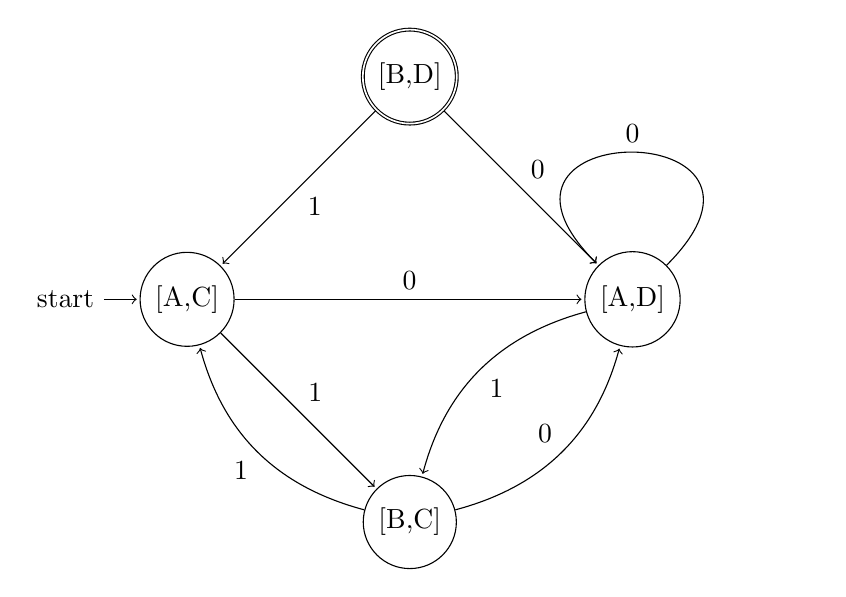
\begin{tikzpicture}[shorten >=1pt,node distance=4cm,on grid,auto]  
   \node[state,initial] (AC)  {[A,C]};

   \node [state,accepting] (BD) [above right= of AC] {[B,D]};
      \node [state] (AD) [below right= of BD] {[A,D]};
   \node [state] (BC) [below right= of AC] {[B,C]};
    \path[->] 
    (AC) edge node {1} (BC)
         edge node {0} (AD)
    (BC) edge [bend right] node {0} (AD)
         edge [bend left] node {1} (AC)
    (AD) edge [loop, above] node {0} ()
         edge [bend right] node {1} (BC)
    (BD) edge node {0} (AD)
         edge node {1} (AC);
\end{tikzpicture}\\

\subsection{Nor}
Once again we can trivially compute the Nor of two languages by switching the final state.
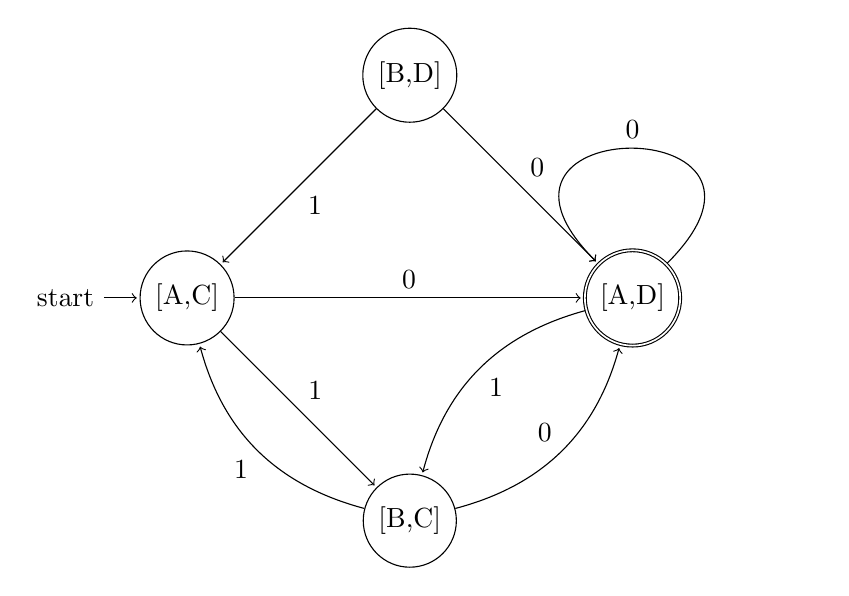
\begin{tikzpicture}[shorten >=1pt,node distance=4cm,on grid,auto]  
   \node[state,initial] (AC)  {[A,C]};

   \node [state] (BD) [above right= of AC] {[B,D]};
      \node [state,accepting] (AD) [below right= of BD] {[A,D]};
   \node [state] (BC) [below right= of AC] {[B,C]};
    \path[->] 
    (AC) edge node {1} (BC)
         edge node {0} (AD)
    (BC) edge [bend right] node {0} (AD)
         edge [bend left] node {1} (AC)
    (AD) edge [loop, above] node {0} ()
         edge [bend right] node {1} (BC)
    (BD) edge node {0} (AD)
         edge node {1} (AC);
\end{tikzpicture}\\

\subsection{Elementary Questions about Regular Languages}

In the same spirit of exploration that permeates this section we can consider some reasonable questions that one might ask about a regular language.\\

A simple question is that of membership, in other words given a regular language $L$ and a string $w$ how can we check if $w \in L$. By constructing the appropriate DFA this becomes a simple problem of sending $w$ through the graph and seeing if it ends at a final state.\\

How can we check if $L = \emptyset$? Once again we can simply construct a DFA and then apply a DFS from the initial state to see if there is any path to the final state.\\

How can we check if $L$ is finite? Construct the DFA and then check if there is a walk from the initial state to the final state that has a cycle. If the walk contains a cycle then the language is infinite, if not its finite.\\

Given regular languages $L_1,L_2$ how can we check if $L_1 = L_2$? Find if $(L_1 \cap \overline{L_2}) \cup (\overline{L_1} \cap L_2) = \emptyset$.
 

\newpage

\section{Non-Regular Languages}

Thus far we have restricted our view to the so called regular languages in order to better understand their intimate connection with various kinds of  tools of computation. Grammars gave as hint that there are in fact more powerful formal systems available, and in turn more expressive languages associated with them. In order to study non-regular languages it is useful to first know how to prove a language is not regular.

\subsection{Detour: The Pigeonhole Principle}

In order to get to the central result of this section we first review the pigeonhole principle and its connection to DFA's. Simply put if there are $n$ pigeons and $m$ pigeon holes with $n > m$ then we know there exists a pigeonhole with at least 2 pigeons.\\

To see how this relates consider the following DFA\\
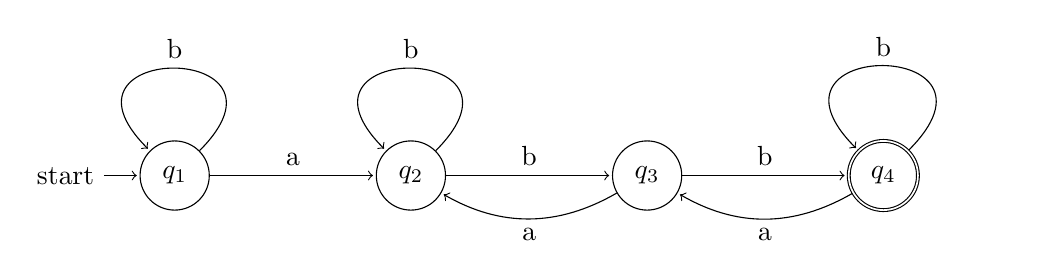
\begin{tikzpicture}[shorten >=1pt,node distance=3cm,on grid,auto]  
   \node[state,initial] (q1)  {$q_1$};
   \node [state] (q2) [right =of q1] {$q_2$};
   \node [state] (q3) [right =of q2] {$q_3$};
   \node [state,accepting] (q4) [right =of q3] {$q_4$};
    \path[->] 
    (q1) edge node {a} (q2)
         edge [loop, above] node {b} ()
    (q2) edge [loop, above] node {b} ()
         edge node {b} (q3)
    (q3) edge [bend left, below] node {a} (q2)
         edge node {b} (q4)
    (q4) edge [loop, above] node {b} ()
         edge [bend left, below] node {a} (q3);
\end{tikzpicture}\\
Now consider that in the walks of strings, $a,aa,aab$ no state is repeated. However for any string of length greater than 4, e.g $aabb, bbaa, abbabb$,  there must be a repeated state by the pigeon hole principle. 

\subsection{The Pumping Lemma}
Consider now a generalization of the previous argument. Take some infinite regular language $L$. Then there exists some DFA that accepts $L$ that has $m$ states. Now let $w \in L$, if $|w| \geq m$ then by the pigeonhole principle a state is repeated in the walk of $w$. Then consider the following diagram\\
\begin{tikzpicture}[shorten >=1pt,node distance=3cm,on grid,auto]  
   \node[state,initial] (q1)  {$x$};
   \node [state] (q2) [right =of q1] {$x$};
   \node [state] (q3) [right =of q2] {$\dots$};
   \node [state] (q4) [right =of q3] {$y$};
   \node [state] (l)  [above =of q4] {$y$};
   \node [state] (l2) [left =of l] {$y$};
   \node [state] (q5) [right =of q4] {$\dots$};
   \node [state,accepting] (q6) [right =of q5] {$z$};
    \path[->] 
    (q1) edge node {} (q2)
    (q2) edge node {} (q3)
    (q3) edge node {} (q4)
    (q4) edge node {} (q5)
         edge [bend right, below] node {} (l)
    (l) edge node {} (l2)
    (l2) edge node {} (q4)
    (q5) edge node {} (q6);
\end{tikzpicture}\\

Then we can decompose the walk into $xyz$, where where $|xy| \leq m$ and   $|y| \geq q|$ as the loop can be a self loop or many states. Notice that we have that $xz, xyz, xyyz, xyyyz, \dots$ are all accepted by the DFA which implies $xy^iz \in L, y \geq 0$. We have just discovered the pumping lemma, put more succinctly.\\

Let $L$ be a infinite regular language then $\exists m, \forall w \in L, |w| \geq m \implies w = xyz, |xy| \leq m, |y| \geq 1$ such that $\forall i \in \mathbb{Z}^+ xy^iz \in L$\\

\subsection{Some Non-Regular Languages}

\begin{theorem}
The language $L = \{a^nb^n | n \geq 0 \}$ is not regular
\end{theorem}

\begin{proof}
Assume for the sake of contradiction that $L$ is regular. Since $L$ is infinite the pumping lemma implies $\exists m, \forall w \in L, |w| \geq m \implies w = xyz$. Let $w = a^mb^m$, then we must have that $xyz = a^mb^m$. But $|xy| \leq m$ so $y = a^k, k \geq 1$. But by the pumping lemma we should have $xy^2z \in L$. Consider that $xy^2z = a^{m+k}b^m$ which is clearly not in $L$ a contradiction so $L$ must not be regular.
\end{proof}

\begin{theorem}
The language $L = \{vv^R | v \in \{a,b\}^* \}$ is not regular
\end{theorem}

\begin{proof}
Assume for the sake of contradiction that $L$ is regular. Since $L$ is infinite the pumping lemma implies $\exists m, \forall w \in L, |w| \geq m \implies w = xyz$. Let $w = a^mb^mb^ma^m$, then we have that $a^mb^mb^ma^m = xyz$ and that $y = a^k, k \geq 1$. By the pumping lemma we should have $xy^2z \in L$. But consider that $xy^2z = a^{m+k}b^mb^ma^m$ which is clearly not in $L$, a contradiction so $L$ must not be regular.
\end{proof}


\begin{theorem}
The language $L = \{a^nb^lc^{n+l} | n,l \geq 0\}$ is not regular
\end{theorem}

\begin{proof}
Assume for the sake of contradiction that $L$ is regular. Since $L$ is infinite the pumping lemma implies $\exists m, \forall w \in L, |w| \geq m \implies w = xyz$. Let $w = a^mb^mc^{2m}$, then we have that $a^mb^mc^{2m} = xyz$ and that $y = a^k, k \geq 1$. By the pumping lemma we should have $xy^0z \in L$. But consider that $xy^0z = a^{m-k}b^mc^{2m}$ which is clearly not in $L$, a contradiction so $L$ must not be regular.
\end{proof}

\begin{theorem}
The language $L = \{a^{n!} | n \geq 0\}$ is not regular
\end{theorem}

\begin{proof}
Assume for the sake of contradiction that $L$ is regular. Since $L$ is infinite the pumping lemma implies $\exists m, \forall w \in L, |w| \geq m \implies w = xyz$. Let $w = a^{m!}$, then we have that $a^{m!} = xyz$ and that $y = a^k, 1 \geq k \leq m$. By the pumping lemma we should have $xy^2z \in L$. Now consider that $xy^2z = a^{m!+k}$, this implies that there must exist a natural number $p$ such that $m! + k = p!$. Now consider that 
\begin{align*}
m! + k &\leq m! + m\\
       &\leq m! + m!\\
       &< mm! + m!\\
       &< m!(m + 1)\\
       &< (m+1)!
\end{align*}
So $m! + k \neq p!$ so $xy^2z \notin L$ a contradiction so $L$ must not be regular.
\end{proof}

\newpage

\section{Context Free Grammars}

We return to grammars in a more unrestricted manner. This time exploring grammars that a not just linear, which allows us to explore languages that are not regular. The richness of context free grammars allow us to express many of the constructs that appear in programming languages making them of fundamental importance to language and compiler design.

Formally we define a context free grammar $G$ as the following 

\begin{center}
$G = (V,T,S,P)$\\
$V:$ Set of variables\\
$T:$ Set of terminal symbols\\
$S:$ Start variable\\
$P:$ Set of Production rules\\
Where productions are of the form\\
$A \rightarrow x, A \in V, x \in \{V,T\}^*$
\end{center}

\subsection{Context Free Languages}
A language $L$ is context free if and only if there is a context free grammar $G$ with $L = L(G)$. As we will later see these languages have their own variants of finite automata that are more powerful than NFA's and DFA's.\\

Ex:
\begin{center}
\begin{align*}
G: S &\rightarrow aSb\\
   S &\rightarrow \lambda\\
\end{align*}
From which we can derive the following string
\begin{align*}
S &\Rightarrow aSb\\
  &\Rightarrow aaSbb\\
  &\Rightarrow aaaSbbb\\
  &\Rightarrow aaabbbb\\
\end{align*}
So we can see that $L(G) = \{a^nb^n | n \geq 0 \}$, a classic non regular language. We can conceptually think of this language as describing match parentheses $((()))$
\end{center}

Ex:
\begin{center}
\begin{align*}
G: S &\rightarrow aSa\\
   S &\rightarrow bSb\\
   S &\rightarrow \lambda\\
\end{align*}
From which we can derive the following string
\begin{align*}
S &\Rightarrow aSa\\
  &\Rightarrow abSba\\
  &\Rightarrow abba\\
\end{align*}
So $L(G) = \{ww^R | w \in \{a,b\}^* \}$ another non regular language.
\end{center}

Ex:
\begin{center}
\begin{align*}
G: S &\rightarrow aSb\\
   S &\rightarrow SS\\
   S &\rightarrow \lambda\\
\end{align*}
From which we can derive the following string
\begin{align*}
S &\Rightarrow SS\\
  &\Rightarrow aSbS\\
  &\Rightarrow abS\\
  &\Rightarrow abaSb\\
  &\rightarrow abab\\
\end{align*}
So $L(G) = \{w | n_a(w) = n_b(w), \text{ and } n_a(v) \geq n_b(v) \text{ in any prefix } v \}$ another non regular language. Conceptually this is a more sophisticated parenthesis matching grammar i.e $()((()))(())$.
\end{center}

As one might have noticed the order of derivation is arbitrary, we could always expand the leftmost or rightmost production.\\

Ex:
\begin{center}
\begin{align*}
S &\rightarrow AB\\
A &\rightarrow aaA\\
A &\rightarrow \lambda\\
B &\rightarrow Bb\\
B &\rightarrow \lambda\\
\end{align*}
Leftmost
\begin{align*}
S &\Rightarrow AB\\
  &\Rightarrow aaAB\\
  &\Rightarrow aaB\\
  &\Rightarrow aaBb\\
  &\Rightarrow aab\\
\end{align*}
Rightmost
\begin{align*}
S &\Rightarrow AB\\
  &\Rightarrow ABb\\
  &\Rightarrow Ab\\
  &\Rightarrow aaAb\\
  &\Rightarrow aab\\
\end{align*}
\end{center}

\subsection{Designing Grammars}

Because of the deep recursion and complex languages grammars can capture it can sometimes be difficult to design them. here we cover some general principles in their design.\\

\subsubsection{Concatenation}
Use separate non terminals to generate disjoint parts of a language and then combine in a production.\\

Ex:
\begin{align*}
G: S &\rightarrow AB\\
   A &\rightarrow aA | \lambda\\
   B &\rightarrow bB | \lambda\\
   L(G) &= a^*b^*\\
\end{align*}

\subsubsection{Closures}
Use recursive productions to generate an arbitrary number of symbols.\\

Ex:
\begin{align*}
A \rightarrow xA | \lambda \text{ Zero or more x's}\\
A \rightarrow yA | y \text{ One or more y's}\\  
\end{align*}

\subsubsection{Matching Constructs}
Write productions which generate strings from the middle.\\\
\begin{align*}
S &\rightarrow aSb | \lambda\\
\{a^nb^n | n \geq 0 \}\\
S \rightarrow aSbb | \lambda\\
\{a^nb^{2n} | n \geq 0 \}\\
\end{align*}

\subsubsection{Union}
Use separate nonterminals for each part of the union and then combine.
\begin{align*}
\{a^n(b^m+c^m) | m > n \geq 0\}\\
\{a^nb^m | m > n \geq 0\} \cup \{a^nc^m | m > n \geq 0\}
\end{align*}

\newpage 
\section{Derivation Trees}
A useful way of visualizing how strings are derived from grammars is the so called "derivation tree".
This representation has the added bonus of being much closer to how we work with grammars in compilers and
helps us define concepts like ambiguity.\\

Ex:
\begin{center}
The tree below derives the string $aab$
\begin{align*}
S &\rightarrow AB\\
A &\rightarrow aaA | \lambda\\
B &\rightarrow Bb | \lambda\\
\end{align*}
\end{center}
\Tree[.S [.A a a [.A $\lambda$ ]]
         [.B [.B $\lambda$ ] b ] ]

Note that we can stop anywhere along the process and build a "partial tree" such partial trees and productions like $aaAB$ are called sentential form.

\subsection{Ambiguity}

In order to understand more precisely what is meant by ambiguity consider the following grammar
\begin{align*}
E &\rightarrow E + E | E*E | (E) | a\\
\end{align*}
Then for the string $a + a*a$ we have two different leftmost derivation trees.\\

\Tree[.E [.E a ] + [.E [.E a ] * [.E a ] ]]
\Tree[.E [.E [.E a ] + [.E a ]] * [.E a ] ]\\

Because of this property we call the above grammar ambiguous.
More formally we define a context free grammar $G$ to be ambiguous if $\exists w \in L(G)$ such that $w$ has two or more leftmost derivations or rightmost derivations.\\

While we deal with ambiguity in natural language with ease, it is not desirable in many places such as a programming language. Consider that in the previous example if we let $a=2$ then for the left tree we get $2+2*2 = 6$ and for the right we get $2+2*2=8$, clearly violating our usual rules of arithmetic.\\

While it often produces less intuitive grammars we can fix the ambiguity. Consider the following
\begin{align*}
E &\rightarrow E + T | T\\
T &\rightarrow T * F | F\\
F &\rightarrow (E) | a\\
\end{align*}
Then we have a new unique derivation tree for $a + a*a$ given by \\

\Tree [.E [.E [.T [.F a ]]] + [.T [.T [.F a ]] * [.F a ]]]

Ex:
\begin{center}
Consider the following grammar
\begin{align*}
\{a^nb^m | m > n \geq 0 \} \cup \{a^nc^m | m > n \geq 0 \}\\
S &\rightarrow T | U\\
T &\rightarrow aTb | Tb | b\\
U &\rightarrow aUc | Uc | c\\
\end{align*}
Which is ambiguous because $abbb$ has two different parse trees. We could try the following fix
\begin{align*}
S &\rightarrow T | U\\
T &\rightarrow aTb | bT | b\\
U &\rightarrow aUc | cU | c\\
\end{align*}
which is no longer ambiguous but generates invalid strings like $babb$. The following grammar solves this problem
\begin{align*}
S &\rightarrow T | V\\
T &\rightarrow aTb | U\\
U &\rightarrow Ub | b\\
V &\rightarrow aVc | W\\
W &\rightarrow Wc | c\\
\end{align*}
\end{center}

Another classic example of an unambiguous grammar comes from the "if-then-else" construct and is sometimes called the "dangling else" problem. Consider the following grammar
\begin{center}
IF\_STMT $\rightarrow$ if EXPR then STMT | if EXPR then STMT else  STMT
\end{center}
Now consider parsing "If expr1 then if expr2 then stmt1 else stmt2"
which has the following parse trees\\
\includegraphics[scale=0.5]{dangling.png}\\

Clearly not all grammars are ambiguous, but it is interesting to ask whether or not there exists languages that are inherently ambiguous. The answer is yes, and we can see this by consider the following grammar
\begin{align*}
L &= \{a^nb^nc^n\} \cup \{a^nb^mc^m\}\\
S &\rightarrow S_1 | S_2\\
S_1 &\rightarrow S_1c | A\\
S_2 &\rightarrow aS_2 | B\\
A &\rightarrow aAb | \lambda\\
B &\rightarrow bBc | \lambda\\
\end{align*}

\subsection{Parsing}

When working with grammars on the theoretical level we can abstract away the details of how strings are accepted by the grammar. However it is a worthwhile endeavor to consider what algorithms exist for deriving strings from a grammar.\\

The naive algorithm is simply an exhaustive search of the grammars productions. Consider the following example for deriving $aabb$
\begin{align*}
S &\rightarrow SS | aSb | bSa | \lambda
\end{align*}
First we find all derivations of length 1
\begin{align*}
S &\Rightarrow SS\\
S &\Rightarrow aSb\\
&\cancel{S \Rightarrow bSa}\\
&\cancel{S \Rightarrow \lambda}\\
\end{align*}

\begin{align*}
S &\Rightarrow SS \Rightarrow SSS\\
S &\Rightarrow SS \Rightarrow aSbS\\
&\cancel{S \Rightarrow SS \Rightarrow bSaS}\\
S &\Rightarrow SS \Rightarrow S\\
S &\Rightarrow aSb \Rightarrow aSSb\\
S &\Rightarrow aSb \Rightarrow aaSbb\\
&\cancel{S \Rightarrow aSb \Rightarrow abSab}\\
&\cancel{S \Rightarrow aSb \Rightarrow ab}\\
\end{align*}
And we can derive $aabb$ from $S \Rightarrow aSb \Rightarrow aaSbb \Rightarrow aabb$. However as the name implies exhaustive search is very slow. If there are no productions of the form 
\begin{align*}
A &\rightarrow B\\
A &\rightarrow \lambda\\
\end{align*}
And we have a string of length $w$ and $k$ productions then we it takes $O(k^w)$ time to parse.\\

If we restrict the form of the grammar we can yield linear time parsing from the exhaustive search. We define an "s grammar" as
\begin{center}
Productions of the form $A \rightarrow ax, a \in T, x \in V^*$\\
and the pair $(A,a)$ appears once
\end{center}
This restriction means that at each phase there is only one possible choice for parsing, so the time is simply the length of the string.\\

We will later show that for general context free grammars there exists a parsing algorithm that parses a string $|w|$ in $O(|w|^3)$ time.


\newpage

\section{Simplifications of Context Free Grammars}

In order to produce a more efficient parsing algorithm we must first derive some rules to simplify grammars into a form that are easier to process.

\subsection{Substitutions}

Consider the following grammar
\begin{align*}
S &\rightarrow aB\\
A &\rightarrow aaA\\
A &\rightarrow abBc\\
B &\rightarrow aA\\
B &\rightarrow b\\
\end{align*}
Then we can easily see that we can remove the production $B \rightarrow b$ and get the following equivalent grammar.
\begin{align*}
S &\rightarrow aB | ab\\
A &\rightarrow aaA\\
A &\rightarrow abBc | abbc\\
B &\rightarrow aA\\
\end{align*}
We can simply further by getting rid of $B \rightarrow aA$ which yields
\begin{align*}
S &\rightarrow aaA | ab\\
A &\rightarrow aaA\\
A &\rightarrow abaAc | abbc\\
\end{align*}
With this intuition established we can now formally define the substitution rule. 
\begin{center}
For any productions\\
$A \rightarrow xBz$\\
$B \rightarrow y_1$\\
Substituting $B \rightarrow y_1$ yields\\
$A \rightarrow xBz | xy_1z$
\end{center}

\subsection{Nullable Variables}

In order to keep the grammar as simple as possible we will derive a rule for removing lambdas from the grammar. We call any production of the form $A \rightarrow \lambda$ a lambda production and any variable $A \Rightarrow \cdots \Rightarrow \lambda$ a nullable variable.\\

Now consider the following grammar 
\begin{align*}
S &\rightarrow aMb\\
M &\rightarrow aMb\\
M &\rightarrow \lambda\\
\end{align*}
Then we can get rid of the lambda production by substitution and get the following grammar
\begin{align*}
S &\rightarrow aMb | ab\\
M &\rightarrow aMb | ab\\
\end{align*}

\subsection{Unit Productions}
Another troublesome situation we need to avoid is productions that loop into each other. We call any production of the form
$A \rightarrow B$ a unit production. Note that we can remove any productions of the form $A \rightarrow A$ immediately.

\subsection{Useless Productions}
We also define two kinds of useless productions.
Any production of the form $A \rightarrow aA$ never terminates and can be removed. We can also remove any productions that are not reachable from the starting production. In general 

\begin{center}
if $S \Rightarrow \dots \Rightarrow xAy \Rightarrow \dots \Rightarrow w, w \in L(G)$\\
then $A$ is useful otherwise its useless.\\
\end{center}
Note that any production is useless if any of its variables are useless.\\

Ex:
\begin{center}
\begin{align*}
S &\rightarrow aS | A | C\\
A &\rightarrow a\\
B &\rightarrow aa\\
C &\rightarrow aCb\\
\end{align*}
Can be transformed into 
\begin{align*}
S &\rightarrow aS | a \\
\end{align*}
\end{center}

\newpage

\section{Chomsky Normal Form}

The Chomsky Normal Form (CNF) is another transformation of grammar that is essential to efficient parsing. Fist we remove all nullable variables, unit productions, and useless variables. Then a CNF is a grammar where are productions are of the form
\begin{align*}
A \rightarrow BC\\
\text{or}\\
A \rightarrow a\\
\end{align*}

Ex:
\begin{center}
The grammar on the left is in CNF and the grammar on the right is not
\begin{align*}
S &\rightarrow AS & S &\rightarrow AS\\
S &\rightarrow a & S &\rightarrow AAS\\
S &\rightarrow SA & S &\rightarrow SA\\
S &\rightarrow b & S &\rightarrow aa\\
\end{align*}
\end{center}

Ex:
\begin{center}
We can transform the following grammar into CNF
\begin{align*}
S \rightarrow ABa\\
A \rightarrow aab\\
B \rightarrow Ac\\
\end{align*}
By introducing variables for terminals and breaking productions up we produce the following CNF
\begin{align*}
S &\rightarrow AV_1\\
V_1 &\rightarrow BT_a\\
A &\rightarrow T_aV_2\\
V_2 &\rightarrow T_aT_b\\
B &\rightarrow AT_c\\
T_a &\rightarrow a\\
T_b &\rightarrow b\\
T_c &\rightarrow c\\
\end{align*}
\end{center}

In general for any CFG that doesnt produce $\lambda$ we can obtain a CNF by the following procedure.

\begin{enumerate}
\item Remove useless productions and variables\\
\item Remove nullable variables\\
\item Remove unit productions\\
\item For every production $a$\\
\begin{enumerate}
\item add production $T_a \rightarrow a$\\
\item In productions: replace $a$ with $T_a$\\
\end{enumerate}
\item Replace any production $A \rightarrow C_1C_2\dots C_n$ with \begin{align*}
A &\rightarrow C_1V_1\\
V_1 &\rightarrow C_2V_2\\
\dots\\
V_{n-2} &\rightarrow C_{n-1}V_n\\
\end{align*}
\end{enumerate}

\newpage


\section{CYK Algorithm}

With a way to transform grammars to CNF we can derive an efficient algorithm for parsing grammars. The algorithm works bottom up and leverages the fact that each production can be split into two parts in order to derive a string in polynomial time. The algorithm is due to Cocke, Younger, and Kasami. The pseudocode for the algorithm is as follows
\begin{lstlisting}[mathescape=true]
let the input be a string I consisting of n characters: $a_1 ... a_n$.
let the grammar contain r nonterminal symbols $R_1 ... R_r$, with start symbol $R_1$.
let P[n,n,r] be an array of booleans. Initialize all elements of P to false.
for each s = 1 to n
  for each unit production $R_v \rightarrow  a_s$
    set P[1,s,v] = true
for each l = 2 to n -- Length of span
  for each s = 1 to n-l+1 -- Start of span
    for each p = 1 to l-1 -- Partition of span
      for each production $R_a  \rightarrow R_bR_c$
        if P[p,s,b] and P[l-p,s+p,c] then set P[l,s,a] = true
if P[n,1,1] is true then
  I is member of language
else
  I is not member of language
\end{lstlisting}

There are $O(|w|^2)$ cells in the table and for each cell it takes $O(|w|)$ to fill in each cell. So given a string of length $|w|$ the algorithm runs in time $O(|w|^3)$ one of the most asymptotically efficient methods for parsing grammars.

Ex:
\begin{center}
Consider the following grammar and the string $w = acbb$
\begin{align*}
S &\rightarrow AB | AC\\
A &\rightarrow AC | AB | a\\
B &\rightarrow BB | BC | b\\
C &\rightarrow AC | CC | c | b\\
\end{align*}
We start with strings of length 1\\
\begin{tabular}{| l | l | r | r |}
\hline
$A$ &  & & \\ 
\hline
 & $C$ &  & \\
\hline 
 & & $B,C$ & \\
\hline 
 & & & $B,C$\\
\hline
\end{tabular}\\
\begin{tabular}{| l | l | r | r |}
\hline
$A$ & $S,A,C$ & & \\ 
\hline
 & $C$ & $C$  & \\
\hline 
 & & $B,C$ & $B,C$ \\
\hline 
 & & & $B,C$\\
\hline
\end{tabular}\\
\begin{tabular}{| l | l | r | r |}
\hline
$A$ & $S,A,C$ & $S,A,C$ & $S,A,C$ \\ 
\hline
 & $C$ & $C$  & $C$ \\
\hline 
 & & $B,C$ & $B,C$ \\
\hline 
 & & & $B,C$\\
\hline
\end{tabular}\\
Since $S$ is in the upper corner $w$ is in the language.
\end{center}

\newpage

\section{Pushdown Automata}

We now return to the world of automata but this time with an increase in computational power. In order to match the computational power of context free grammars, we must imbue automata with some simple memory. Conceptually PDA's are like NFA's or DFA's but each state has a stack that can be used as a simple memory.\\

Formally we define a Non deterministic Pushdown Automata (NPDA) as
\begin{center}
$M = (Q,\Sigma,\Gamma,\delta,q_0,z,F)$\\
$Q :$ set of states\\
$\Sigma :$ input alphabet\\
$\Gamma :$ stack alphabet\\
$\delta : Q \times (\Sigma \cup \{\lambda\}) \times \Gamma$ transition function\\
$q_0 :$ initial state\\
$z \in \Gamma :$ stack start symbol\\
$F :$ set of final states\\
\end{center}

We denote the rules for the stack as $a,b ; c$ where $a$ is the character read, $b$ is the character to take off the stack, and $c$ is the character to be put onto the stack. Notice that we reserve a special symbol to denote the bottom of the stack. If the stack is empty we cannot transition and the machine halts and rejects the input string. 

Ex:
\begin{center}
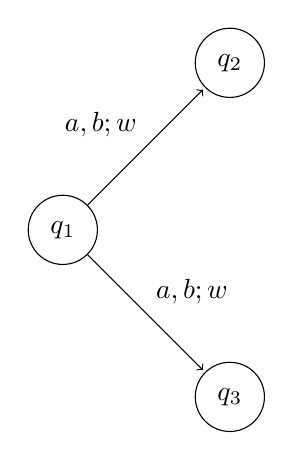
\begin{tikzpicture}[shorten >=1pt,node distance=3cm,on grid,auto]  
   \node[state] (q1)  {$q_1$};
   \node [state] (q2) [above right =of q1] {$q_2$};
   \node [state] (q3) [below right =of q1] {$q_3$};
    \path[->] 
    (q1) edge node  {$a,b ; w$} (q2)
         edge node  {$a,b ; w$} (q3);
\end{tikzpicture}\\
This NPDA has the transition function $\delta(q_1,a,b) = \{(q_2,w), (q_3,w)\}$
\end{center}

For convenience we can define the instantaneous description $(q,u,s)$ where $q$ is the current state, $u$ is the remaining input, an $s$ is the current stack content. We can chain together these computations using the $\vdash$.\\

Ex:
\begin{center}
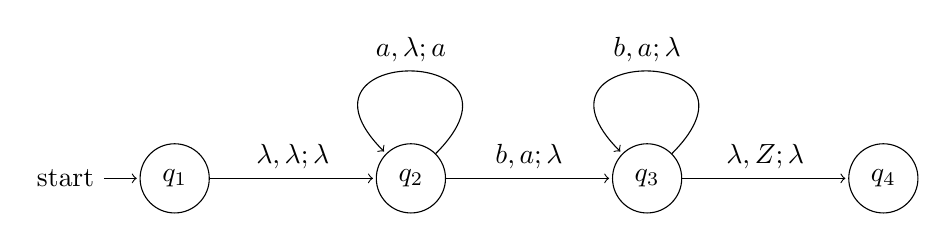
\begin{tikzpicture}[shorten >=1pt,node distance=3cm,on grid,auto]  
   \node[state, initial] (q1)  {$q_1$};
   \node [state] (q2) [right =of q1] {$q_2$};
   \node [state] (q3) [right =of q2] {$q_3$};
   \node [state] (q4) [right =of q3] {$q_4$};
    \path[->] 
    (q1) edge node  {$\lambda,\lambda ; \lambda$} (q2)
    (q2) edge [loop,above] node  {$a,\lambda ; a$} ()
         edge node  {$b,a ; \lambda$} (q3)
    (q3) edge node  {$\lambda,Z ; \lambda$} (q4)
         edge [loop,above] node  {$b,a ; \lambda$} ();
\end{tikzpicture}\\
\begin{align*}
(q_0,aaabbb,Z) &\vdash (q_1,aaabbb,Z)\\
&\vdash (q_1,aabbb,aZ)\\
&\vdash (q_1,abbb,aaZ)\\
&\vdash (q_1,bbb,aaaZ)\\
&\vdash (q_2,bb,aaZ)\\
&\vdash (q_2,b,aZ)\\
&\vdash (q_2,\lambda,Z)\\
&\vdash (q_3,\lambda,Z)\\
\end{align*}
More conveniently we can write $(q_0,aaabbb,Z) \stackrel{*}{\vdash} (q_3,\lambda,Z)$
\end{center}

Note that a string is accepted if the input is completely consumed and the last state is a final state, the contents of the stack have no affect on whether or not the string is accepted.
Formally the language of an NPDA $M$ is
\begin{align*}
L(M) = \{ w | (q_0,w,s) \stackrel{*}{\vdash} (q_f,\lambda,s') \}
\end{align*}



\subsection{NPDA = CFG}

We can now proceed to a central result of the theory of NPDA's, their equivalence between context free grammars and NPDA's.

\begin{theorem}
Let $CFG = \{ \text{Context free languages} \}$ and $NPDA = \{ \text{NPDA languages} \}$ then $CFG = NPDA$
\end{theorem}

\begin{proof}
Let $x \in CFG$, then $x$ has a context free grammar that we will simulate of leftmost derivation by the following construction.

\begin{center}
For any production $A \rightarrow w$ and for any terminal $a$ we construct the following $NPDA$\\
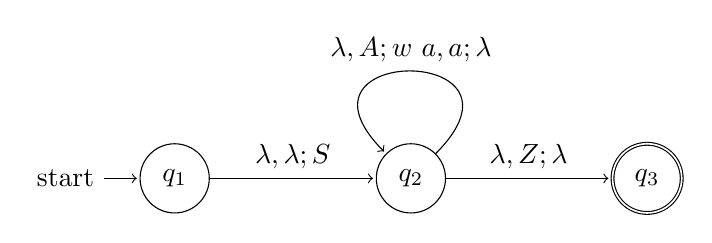
\begin{tikzpicture}[shorten >=1pt,node distance=3cm,on grid,auto]  
   \node[state, initial] (q1)  {$q_1$};
   \node [state] (q2) [right =of q1] {$q_2$};
   \node [state,accepting] (q3) [right =of q2] {$q_3$};
    \path[->] 
    (q1) edge node  {$\lambda,\lambda ; S$} (q2)
    (q2) edge [loop,above] node  {$\lambda, A; w \ a,a ; \lambda$} ()
         edge node  {$\lambda,Z ; \lambda$} (q3);
\end{tikzpicture}\\
\end{center} 

Then and string in the grammar is also recognized by the $NPDA$ and we have that $CFG \subseteq NPDA$. The reverse direction is so contrived it has been omitted from the class.
\end{proof}


\subsection{DPDA v.s NPDA}

Unlike the finite automata we studied earlier non determinism actually buys us more computational power for push down automata. The languages recognized by NPDA's are richer than those recognized by DPDA's. We first note some subtleties of DPDA's.

\begin{center}
The following transitions are allowed in DPDA's\\
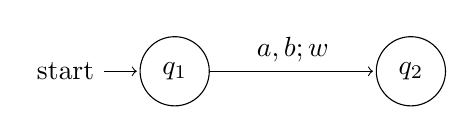
\begin{tikzpicture}[shorten >=1pt,node distance=3cm,on grid,auto]  
   \node[state, initial] (q1)  {$q_1$};
   \node [state] (q2) [right =of q1] {$q_2$};
    \path[->] 
    (q1) edge node  {$a,b ; w$} (q2);
\end{tikzpicture}\\
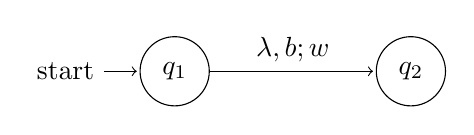
\begin{tikzpicture}[shorten >=1pt,node distance=3cm,on grid,auto]  
   \node[state, initial] (q1)  {$q_1$};
   \node [state] (q2) [right =of q1] {$q_2$};
    \path[->] 
    (q1) edge node  {$\lambda,b ; w$} (q2);
\end{tikzpicture}\\
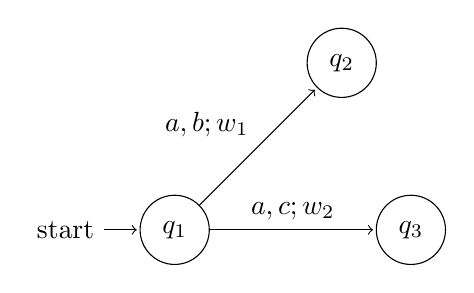
\begin{tikzpicture}[shorten >=1pt,node distance=3cm,on grid,auto]  
   \node[state, initial] (q1)  {$q_1$};
   \node [state] (q2) [above right =of q1] {$q_2$};
   \node [state] (q3) [right =of q1] {$q_3$};
    \path[->] 
    (q1) edge node  {$a,b ; w_1$} (q2)
         edge node  {$a,c ; w_2$} (q3);
\end{tikzpicture}\\
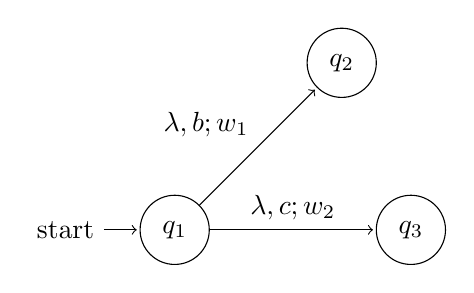
\begin{tikzpicture}[shorten >=1pt,node distance=3cm,on grid,auto]  
   \node[state, initial] (q1)  {$q_1$};
   \node [state] (q2) [above right =of q1] {$q_2$};
   \node [state] (q3) [right =of q1] {$q_3$};
    \path[->] 
    (q1) edge node  {$\lambda,b ; w_1$} (q2)
         edge node  {$\lambda,c ; w_2$} (q3);
\end{tikzpicture}\\
But the following are non deterministic and not allowed\\
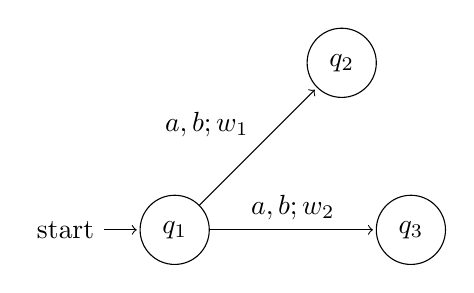
\begin{tikzpicture}[shorten >=1pt,node distance=3cm,on grid,auto]  
   \node[state, initial] (q1)  {$q_1$};
   \node [state] (q2) [above right=of q1] {$q_2$};
   \node [state] (q3) [right =of q1] {$q_3$};
    \path[->] 
    (q1) edge node  {$a,b ; w_1$} (q2)
         edge node  {$a,b ; w_2$} (q3);
\end{tikzpicture}\\
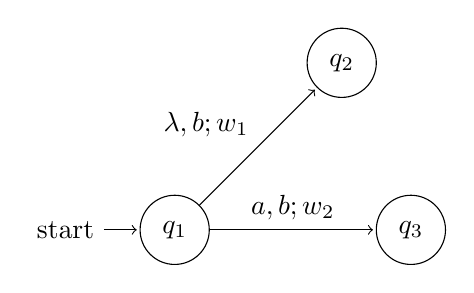
\begin{tikzpicture}[shorten >=1pt,node distance=3cm,on grid,auto]  
   \node[state, initial] (q1)  {$q_1$};
   \node [state] (q2) [above right =of q1] {$q_2$};
   \node [state] (q3) [right =of q1] {$q_3$};
    \path[->] 
    (q1) edge node  {$\lambda,b ; w_1$} (q2)
         edge node  {$a,b ; w_2$} (q3);
\end{tikzpicture}\\ 
\end{center}

Ex:
\begin{center}
$L(M) = \{a^nb^n | n \geq 0 \}$\\
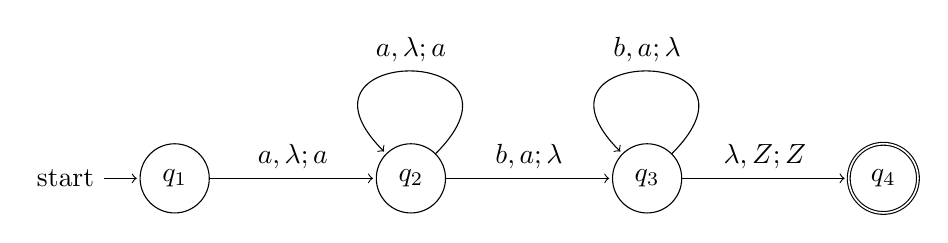
\begin{tikzpicture}[shorten >=1pt,node distance=3cm,on grid,auto]  
   \node[state, initial] (q1)  {$q_1$};
   \node [state] (q2) [right=of q1] {$q_2$};
   \node [state] (q3) [right =of q2] {$q_3$};
   \node [state,accepting] (q4) [right =of q3] {$q_4$};
    \path[->] 
    (q1) edge node  {$a, \lambda; a$} (q2)
    (q2) edge [loop,above] node {$a, \lambda; a$} ()
         edge node {$b,a ; \lambda$} (q3)
    (q3) edge [loop,above] node {$b, a; \lambda$} ()
         edge node {$\lambda, Z; Z$} (q4);
\end{tikzpicture}\\
\end{center}

A simple language which cannot be recognized by a DPDA is $L = {ww^R}$ consider the following NPDA that recognizes it
\begin{center}
$L(M) = \{a^nb^n | n \geq 0 \}$\\
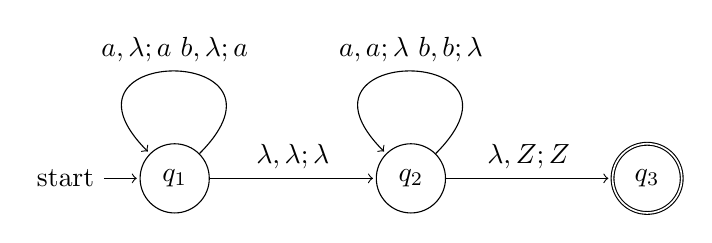
\begin{tikzpicture}[shorten >=1pt,node distance=3cm,on grid,auto]  
   \node[state, initial] (q1)  {$q_1$};
   \node [state] (q2) [right=of q1] {$q_2$};
   \node [state,accepting] (q3) [right =of q2] {$q_3$};
    \path[->] 
    (q1) edge [loop,above] node  {$a, \lambda; a \ b, \lambda; a$} ()
         edge  node  {$\lambda, \lambda ; \lambda$} (q2)
    (q2) edge [loop,above] node {$a, a; \lambda \ b, b ; \lambda$} ()
         edge node {$\lambda, Z ; Z$} (q3);
\end{tikzpicture}\\
\end{center}

We will now rigorously prove this idea.

\begin{theorem}
Let $DPDA = \{ \text{Languages accepted by DPDA's} \}$ and $NPDA = \{ \text{Languages accepted by NPDA's} \}$, then $DPDA \subset NPDA$.
\end{theorem}

\begin{proof}
Consider the language $L = \{a^nb^n\} \cup \{a^nb^{2n}\} \ n \geq 0$ then we have the following CFG
\begin{align*}
S &\rightarrow S_1 | S_2\\
S_1 &\rightarrow aS_1b | \lambda\\
S_2 &\rightarrow aS_2bb | \lambda\\  
\end{align*}
so $L \in NPDA$. Now assume for a contradiction that there is a DPDA $M$ that accepts $L$. Then $M$ would be of the following form
\begin{center}
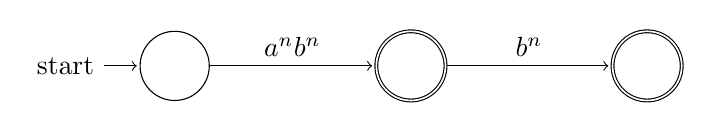
\begin{tikzpicture}[shorten >=1pt,node distance=3cm,on grid,auto]  
   \node[state, initial] (q1)  {};
   \node [state,accepting] (q2) [right=of q1] {};
   \node [state,accepting] (q3) [right =of q2] {};
    \path[->] 
    (q1) edge node  {$a^nb^n$} (q2)
    (q2) edge node {$b^n$} (q3);
\end{tikzpicture}\\
\end{center}
We will now take the following as facts but will prove it later. The language $N = a^nb^nc^n$ and $L \cup N$ are not context free. But if $M$ were to exist we could construct the following
\begin{center}
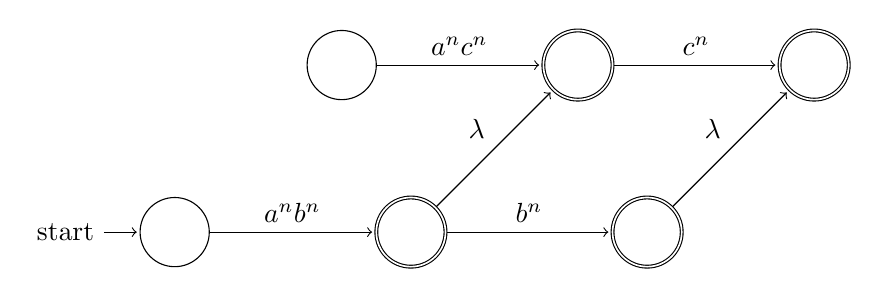
\begin{tikzpicture}[shorten >=1pt,node distance=3cm,on grid,auto]  
   \node[state, initial] (q1)  {};
   \node [state,accepting] (q2) [right=of q1] {};
   \node [state,accepting] (q3) [right =of q2] {};
   \node [state] (q4)  [above right=of q1] {};
   \node [state,accepting] (q5) [right =of q4] {};
   \node [state,accepting] (q6) [right =of q5] {};
    \path[->] 
    (q1) edge node  {$a^nb^n$} (q2)
    (q2) edge node {$b^n$} (q3)
         edge node {$\lambda$} (q5)
    (q4) edge node  {$a^nc^n$} (q5)
    (q5) edge node {$c^n$} (q6)
    (q3) edge node {$\lambda$} (q6);
\end{tikzpicture}\\
\end{center}
Which would imply that $L \cup N$ is context free a contradiction.
\end{proof}

\newpage

\section{Pumping Lemma for Context Free Langauges}

Just as the pumping lemma for regular languages helped us discern from those that were reqular and those that were not, we can develop a similar lemma for context free languages. While similar the complexity of context free languages requires we take some extra subtleties into account.


Let $L$ be an infinite context free language. Let $G$ be the grammar of $L - \{\lambda\}$ and remove any unit or lambda productions from $G$. Now let $w \in L(G)$ with length $|w|\geq m$. Now consider the derivation of $w$
\begin{align*}
S \Rightarrow \dots a_1Aa_2 \Rightarrow \dots a_3Aa_4 \dots w
\end{align*} 
And notice that some variable must be repeated. In terms of a derivation tree we can visualize this as\\
\Tree[.S \qroof{u}. [.A \qroof{v}. A \qroof{y}. ] \qroof{z}. ]
Where $u,v,x,y,z$ are strings of terminals. Then we have the following possible derivations
\begin{align*}
S &\stackrel{*}{\Rightarrow} uAz\\
A &\stackrel{*}{\Rightarrow} vAy\\
A &\stackrel{*}{\Rightarrow} x\\
\end{align*}
This immediately implies that $S \stackrel{*}{\Rightarrow} uAz \stackrel{*}{\Rightarrow} uxz$
in other words $uv^0xy^0z \in L(G)$. And by the same arguments $uv^1xy^1z,uv^2xy^2z \in L(G)$. In fact $\forall i \geq 0, uv^ixy^iz \in L(G)$. Note that we have $|vxy| \leq m$ since $w \geq m$ and $A$ is the last repeated variable. We also have that $|vy| \geq 1$ since there are no unit or $\lambda$ productions. We have just derived the pumping lemma for CFL's.\\

\begin{theorem}
Let $L$ be an infinite context free language, then there exists $m \in \mathbb{N}$ such that $\forall w \in L, |w| \geq m$ implies that we can rewrite $w = uvxyz$ with lengths $|vxy| \leq m$ and $|vy| \geq 1$. Furthermore we have that $\forall i \geq 0, uv^ixy^iz \in L$
\end{theorem} 

\subsection{Using the pumping lemma}
With the pumping lemma established we can now explore some languages that are not context free. 


\begin{theorem}
$L = \{a^nb^nc^n | n \geq 0\}$ is not context free.
\end{theorem}
\begin{proof}
 Assume for sake of contradiction that it were then we could apply the pumping lemma to the string $w = a^mb^mc^m$. Since its length is clearly greater than $m$ we can rewrite it as $w = uvxyz$ with $|vxy| \leq m$ and $|vy| \geq 1$. Now in order to get  contradiction we must examine all possible locations of $vxy$ in $w$.\\

Case 1: all a's\\
if vxy are all a's then we can write the string as $a^{m-k}a^kb^mc^m$ for $k \geq 1$ pumping up yields $uv^2xy^2z = a^{m+k}b^mc^m$ which is clearly not in $L$ a contradiction. (Notice that when we have all the same character the analysis is essentially the same as the pumping lemma for regular languages)\\

Case 2 : all b's 
if vxy are all b's then we can write the string as $a^mb^{m-k}b^kc^m$ for $k \geq 1$ pumping up yields $uv^2xy^2z = a^mb^{m+k}c^m$ which is clearly not in $L$ a contradiction. \\

Case 3: all c's is a identical argument to case 2 and 3\\

Case 4: mix of a's and b's
if vxy is a mix of a's and b's then we can write the string as $a^{m-k_1}a^{k_1}b^{k_1}b^{m-k_2}b^kc^m$ for $k \geq 1$ pumping up yields $uv^2xy^2z = a^{m+k_1}b^{m+k_2}c^m$ which is clearly not in $L$ a contradiction.\\

A sub case is if $v$ contains $a$'s and $b$'s and $y$ is all $b$'s. Then we can write the string as
$a^{m-k_1}a^{k_1}b^{k_2}b^kb^{m-k_2-k}c^m$ for $k_1 + k_2 + k \geq 1$. pumping up yields 
$uv^2xy^2z = a^mb^{k_2}a^{k_1}b^{m+2k_2+k}c^m$ which is clearly not in $L$ a contradiction.\\

There is another subcase with $v$ containing all $a$' and $y$ containing a mix but the argument is identical.\\

Case 5: mix of b's and c's is a identical argument to case 4\\

Since every case leads to a contradiction we have show that $L$ is not context free.
\end{proof}


\begin{theorem}
$L = \{vv | v \in \{a,b\}^* \}$ is not context free.
\end{theorem}

\begin{proof}
 Assume for sake of contradiction that it were then we could apply the pumping lemma to the string $w = a^mb^ma^mb^m$. Since its length is clearly greater than $m$ we can rewrite it as $w = uvxyz$ with $|vxy| \leq m$ and $|vy| \geq 1$. Now in order to get  contradiction we must examine all possible locations of $vxy$ in $w$.\\

Case 1: all a's\\
if vxy are all a's then we can write the string as $a^{m-k}b^ma^mb^m$ for $k \geq 1$ pumping up yields $uv^2xy^2z = a^{m+k}b^ma^mb^m$ which is clearly not in $L$ a contradiction. 

Case 2 : mix of a's and b's
if $v$ overlaps the first $a^mb^m$ and $y$ overlaps the first $b^m$ then we can write the string as $a^{m-k_1}a^{k_1}b^{k_2}b^{k_3}b^{m-k_2-k_3}$ for $k_1,k_2 \geq 1$ pumping up yields $uv^2xy^2z = a^mb^{k_2}a^{k_1}b^{m+k_3}a^mb^m$ which is clearly not in $L$ a contradiction. \\

all other cases are identical to either 1 or 2, and since every case leads to a contradiction we have show that $L$ is not context free.
\end{proof}

\newpage

\section{Closure Properties of CFG's}
Before closing our study of context free grammars we will first explore some of the closure properties they have. These properties will also provide some useful tools for proving whether or not a language is context free.

\subsection{Union} 

\begin{theorem}
Let $L_1,L_2$ be context free languages then $L_1 \cup L_2$ is context free
\end{theorem}
\begin{proof}
Let $L_1,L_2$ be context free languages. Then they are described by two grammars $G_1,G_2$. Let $S_1,S_2$ be the starting productions of the grammar. Then we can construct $L_1 \cup L_2$ by simply adding a new start variable $S$ and the production $S \rightarrow S_1 | S_2$.
\end{proof}


\subsection{Concatenation}
\begin{theorem}
Let $L_1,L_2$ be context free languages then $L_1L_2$ is context free
\end{theorem}
\begin{proof}
Let $L_1,L_2$ be context free languages. Then they are described by two grammars $G_1,G_2$. Let $S_1,S_2$ be the starting productions of the grammar. Then we can construct $L_1L_2$ by simply adding a new start variable $S$ and the production $S \rightarrow S_1S_2$.
\end{proof}


\subsection{Star closure}
\begin{theorem}
Let $L$ be a context free language then $L^*$ is context free
\end{theorem}
\begin{proof}
Let $L$ be a context free language. Then it is described by a grammar $G$ with a start variable $S$. Then we can construct $L^*$ by adding a new start variable $S_1$ and the production $S_1 \rightarrow SS_1 | \lambda$.
\end{proof}


\subsection{Negative Closure properties}
Interestingly context free languages are not closed under many of the same operations that regular languages were. 

\subsection{Intersection}
CFG's are not closed under intersection. Consider the following grammars
\begin{align*}
L_1 &= \{a^nb^nc^m | n,m \geq 0\}\\ 
L_2 &= \{a^nb^mc^m | n,m \geq 0\}\\
L_1 \cap L_2 &= \{a^nb^nc^n | n \geq 0\}
\end{align*}
Despite $L_1,L_2$ being context free their intersection is not.

\subsection{Complement}
CFG's are not closed under complement. Assume that CFG's are closed under complement. Consider the following grammars
\begin{align*}
L_1 &= \{a^nb^nc^m | n,m \geq 0\}\\ 
L_2 &= \{a^nb^mc^m | n,m \geq 0\}\\
\overline{L_1 \cup L_2} &= L_1 \cap L_2 = \{a^nb^nc^n | n \geq 0\}
\end{align*}
We can see that this is a contradiction, so CFG's must not be closed under complement.


\subsection{Regular closure}
Despite not being closed under intersection with CFG's we do have closure with CFG's and regular languages.\\

\begin{theorem}
Let $L_1$ be context free and $L_2$ be regular, then $L_1 \cap L_2$ is context free
\end{theorem}
\begin{proof}
Let $L_1$ be context free and $L_2$ be regular, then we can construct an NPDA that recognizes $L_1 \cap L_2$. Let $M_1$ be the NPDA that recognizes $L_1$ and $M_2$ be the DFA that recognizes $L_2$. Now for any arbitrary transition from $M_1,M_2$ we construct the following
\begin{center}
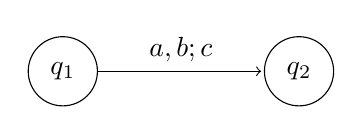
\begin{tikzpicture}[shorten >=1pt,node distance=3cm,on grid,auto]  
   \node [state] (q1)  {$q_1$};
   \node [state] (q2) [right=of q1] {$q_2$};
    \path[->] 
    (q1) edge node  {$a,b;c$} (q2);
\end{tikzpicture}
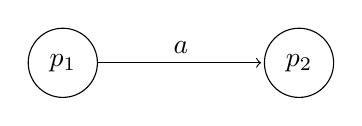
\begin{tikzpicture}[shorten >=1pt,node distance=3cm,on grid,auto]  
   \node [state] (q1)  {$p_1$};
   \node [state] (q2) [right=of q1] {$p_2$};
    \path[->] 
    (q1) edge node  {$a$} (q2);
\end{tikzpicture}\\
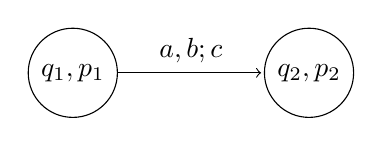
\begin{tikzpicture}[shorten >=1pt,node distance=3cm,on grid,auto]  
   \node [state] (q1)  {$q_1,p_1$};
   \node [state] (q2) [right=of q1] {$q_2,p_2$};
    \path[->] 
    (q1) edge node  {$a,b;c$} (q2);
\end{tikzpicture}
\end{center}

For any lambda transition and empty state
\begin{center}
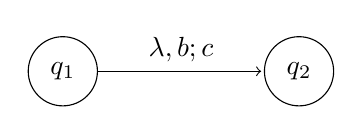
\begin{tikzpicture}[shorten >=1pt,node distance=3cm,on grid,auto]  
   \node [state] (q1)  {$q_1$};
   \node [state] (q2) [right=of q1] {$q_2$};
    \path[->] 
    (q1) edge node  {$\lambda,b;c$} (q2);
\end{tikzpicture}
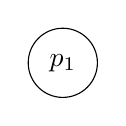
\begin{tikzpicture}[shorten >=1pt,node distance=3cm,on grid,auto]  
   \node [state] (q1)  {$p_1$};
\end{tikzpicture}\\
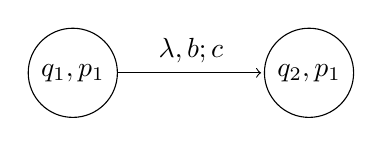
\begin{tikzpicture}[shorten >=1pt,node distance=3cm,on grid,auto]  
   \node [state] (q1)  {$q_1,p_1$};
   \node [state] (q2) [right=of q1] {$q_2,p_1$};
    \path[->] 
    (q1) edge node  {$\lambda,b;c$} (q2);
\end{tikzpicture}
\end{center}

For the initial state
\begin{center}
\begin{tikzpicture}[shorten >=1pt,node distance=3cm,on grid,auto]  
   \node [state,initial] (q1)  {$q_0$};
\end{tikzpicture}
\begin{tikzpicture}[shorten >=1pt,node distance=3cm,on grid,auto]  
   \node [state,initial] (q1)  {$p_0$};
\end{tikzpicture}\\
\begin{tikzpicture}[shorten >=1pt,node distance=3cm,on grid,auto]  
   \node [state,initial] (q1)  {$q_0,p_0$};
\end{tikzpicture}
\end{center}

And for all final states
\begin{center}
\begin{tikzpicture}[shorten >=1pt,node distance=3cm,on grid,auto]  
   \node [state,accepting] (q1)  {$q_1$};
\end{tikzpicture}
\begin{tikzpicture}[shorten >=1pt,node distance=3cm,on grid,auto]  
   \node [state,accepting] (q1)  {$p_1$};
   \node [state,accepting] (q2)  {$p_2$};
\end{tikzpicture}\\
\begin{tikzpicture}[shorten >=1pt,node distance=3cm,on grid,auto]  
   \node [state,accepting] (q1)  {$q_1,p_1$};
   \node [state,accepting] (q2)  {$q_1,p_2$};
\end{tikzpicture}
\end{center}

Which yields a NPDA that recognizes $L_1 \cap L_2$ therefore CFG's are closed under intersection with regular languages.
\end{proof}

\newpage

\section{Turing Machines: The Final Frontier of Computation}
After exploring many different forms of computation we come to turing machines. Despite being a rather simple modification to the NPDA's we saw in the last chapter this gives us a massive leap in computational power.\\

Conceptually a turing machine is the combination of an infinite tape that has a head capable of reading from the cells and writing back to them, combined with a control unit that will be represented similar to other automata\\

\begin{center}
\begin{tikzpicture}
\tikzstyle{every path}=[very thick]

\edef\sizetape{0.7cm}
\tikzstyle{tmtape}=[draw,minimum size=\sizetape]
\tikzstyle{tmhead}=[arrow box,draw,minimum size=.5cm,arrow box
arrows={east:.25cm, west:0.25cm}]

%% Draw TM tape
\begin{scope}[start chain=1 going right,node distance=-0.15mm]
    \node [on chain=1,tmtape,draw=none] {$\ldots$};
    \node [on chain=1,tmtape] {$\diamond$};
    \node [on chain=1,tmtape] (input) {b};
    \node [on chain=1,tmtape] {b};
    \node [on chain=1,tmtape] {a};
    \node [on chain=1,tmtape] {a};
    \node [on chain=1,tmtape] {a};
    \node [on chain=1,tmtape] {a};
    \node [on chain=1,tmtape] {$\diamond$};
    \node [on chain=1,tmtape,draw=none] {$\ldots$};
    \node [on chain=1] {\textbf{Input/Output Tape}};
\end{scope}
\end{tikzpicture}
\end{center}

At each time step the head must read, write, and then move left or right. The diamonds are used to represent empty cells. Note that the read write head always starts at the left most character in the string and that the empty string can never be put on the tape.\\

The control unit transitions have the form\\
\begin{center}
\begin{tikzpicture}[shorten >=1pt,node distance=3cm,on grid,auto]  
   \node [state] (q1)  {$q_1$};
   \node [state] (q2) [right =of q1] {$q_2$};
   \path[->] 
    (q1) edge node  {$a \rightarrow b, L$} (q2);
\end{tikzpicture}\\
\begin{tikzpicture}[shorten >=1pt,node distance=3cm,on grid,auto]  
   \node [state] (q1)  {$q_1$};
   \node [state] (q2) [right =of q1] {$q_2$};
   \path[->] 
    (q1) edge node  {$a \rightarrow b, R$} (q2);
\end{tikzpicture}
\end{center}


Note that we do not allow lambda transitions, but we do allow the transitions to be partial like in the following
\begin{center}
\begin{tikzpicture}
\tikzstyle{every path}=[very thick]

\edef\sizetape{0.7cm}
\tikzstyle{tmtape}=[draw,minimum size=\sizetape]
\tikzstyle{tmhead}=[arrow box,draw,minimum size=.5cm,arrow box
arrows={east:.25cm, west:0.25cm}]

%% Draw TM tape
\begin{scope}[start chain=1 going right,node distance=-0.15mm]
    \node [on chain=1,tmtape,draw=none] {$\ldots$};
    \node [on chain=1,tmtape] {$\diamond$};
    \node [on chain=1,tmtape] {$\diamond$};
    \node [on chain=1,tmtape] {a};
    \node [on chain=1,tmtape] {b};
    \node [on chain=1,tmtape] {a};
    \node [on chain=1,tmtape] (input) {c};
    \node [on chain=1,tmtape] {$\diamond$};
    \node [on chain=1,tmtape] {$\diamond$};
    \node [on chain=1,tmtape,draw=none] {$\ldots$};
\end{scope}
\node [tmhead,yshift=-.3cm] at (input.south) (head) {$q_1$};
\end{tikzpicture}\\
\begin{tikzpicture}[shorten >=1pt,node distance=3cm,on grid,auto]  
   \node [state] (q1)  {$q_1$};
   \node [state] (q2) [above right =of q1] {$q_2$};
   \node [state] (q3) [below right =of q1] {$q_2$};
   \path[->] 
    (q1) edge node  {$a \rightarrow b, R$} (q2)
         edge node {$b \rightarrow d, L$} (q3);
         
\end{tikzpicture}
\end{center}
Note that there is nowhere to go on the input c in which case we say the machine halts.\\

Another tweak to our turing machines is that we can have multiple final states, but unlike our old automata we cannot have transitions out of final states. A final subtlety to note is that a turing machine accepts a string if it halts in a final state. But a turing machine can reject the input if it halts in a non final state or enters a infinite loop.\\

Ex:
\begin{center}
A turing machine that accepts the language $aa^*$\\
\begin{tikzpicture}[shorten >=1pt,node distance=3cm,on grid,auto]  
   \node [state,initial] (q1)  {$q_1$};
   \node [state,accepting] (q2) [right of=q1]  {$q_2$};
   \path[->] 
    (q1) edge [loop,above] node  {$a \rightarrow a, R$} ()
         edge node {$\diamond \rightarrow \diamond, L$} (q2);      
\end{tikzpicture}\\
\begin{tikzpicture}
\tikzstyle{every path}=[very thick]

\edef\sizetape{0.7cm}
\tikzstyle{tmtape}=[draw,minimum size=\sizetape]
\tikzstyle{tmhead}=[arrow box,draw,minimum size=.5cm,arrow box
arrows={east:.25cm, west:0.25cm}]
\begin{scope}[start chain=1 going right,node distance=-0.15mm]
    \node [on chain=1,tmtape,draw=none] {$\ldots$};
    \node [on chain=1,tmtape] {$\diamond$};
    \node [on chain=1,tmtape] {$\diamond$};
    \node [on chain=1,tmtape] (input) {a};
    \node [on chain=1,tmtape] {a};
    \node [on chain=1,tmtape] {a};
    \node [on chain=1,tmtape] {$\diamond$};
    \node [on chain=1,tmtape] {$\diamond$};
    \node [on chain=1,tmtape,draw=none] {$\ldots$};
\end{scope}
\node [tmhead,yshift=-.3cm] at (input.south) (head) {$q_1$};
\end{tikzpicture}\\
\begin{tikzpicture}
\tikzstyle{every path}=[very thick]

\edef\sizetape{0.7cm}
\tikzstyle{tmtape}=[draw,minimum size=\sizetape]
\tikzstyle{tmhead}=[arrow box,draw,minimum size=.5cm,arrow box
arrows={east:.25cm, west:0.25cm}]
\begin{scope}[start chain=1 going right,node distance=-0.15mm]
    \node [on chain=1,tmtape,draw=none] {$\ldots$};
    \node [on chain=1,tmtape] {$\diamond$};
    \node [on chain=1,tmtape] {$\diamond$};
    \node [on chain=1,tmtape]  {a};
    \node [on chain=1,tmtape] (input) {a};
    \node [on chain=1,tmtape] {a};
    \node [on chain=1,tmtape] {$\diamond$};
    \node [on chain=1,tmtape] {$\diamond$};
    \node [on chain=1,tmtape,draw=none] {$\ldots$};
\end{scope}
\node [tmhead,yshift=-.3cm] at (input.south) (head) {$q_1$};
\end{tikzpicture}\\
\begin{tikzpicture}
\tikzstyle{every path}=[very thick]

\edef\sizetape{0.7cm}
\tikzstyle{tmtape}=[draw,minimum size=\sizetape]
\tikzstyle{tmhead}=[arrow box,draw,minimum size=.5cm,arrow box
arrows={east:.25cm, west:0.25cm}]
\begin{scope}[start chain=1 going right,node distance=-0.15mm]
    \node [on chain=1,tmtape,draw=none] {$\ldots$};
    \node [on chain=1,tmtape] {$\diamond$};
    \node [on chain=1,tmtape] {$\diamond$};
    \node [on chain=1,tmtape] {a};
    \node [on chain=1,tmtape] {a};
    \node [on chain=1,tmtape] (input) {a};
    \node [on chain=1,tmtape] {$\diamond$};
    \node [on chain=1,tmtape] {$\diamond$};
    \node [on chain=1,tmtape,draw=none] {$\ldots$};
\end{scope}
\node [tmhead,yshift=-.3cm] at (input.south) (head) {$q_1$};
\end{tikzpicture}\\
\begin{tikzpicture}
\tikzstyle{every path}=[very thick]

\edef\sizetape{0.7cm}
\tikzstyle{tmtape}=[draw,minimum size=\sizetape]
\tikzstyle{tmhead}=[arrow box,draw,minimum size=.5cm,arrow box
arrows={east:.25cm, west:0.25cm}]
\begin{scope}[start chain=1 going right,node distance=-0.15mm]
    \node [on chain=1,tmtape,draw=none] {$\ldots$};
    \node [on chain=1,tmtape] {$\diamond$};
    \node [on chain=1,tmtape] {$\diamond$};
    \node [on chain=1,tmtape] {a};
    \node [on chain=1,tmtape] {a};
    \node [on chain=1,tmtape] {a};
    \node [on chain=1,tmtape] (input) {$\diamond$};
    \node [on chain=1,tmtape] {$\diamond$};
    \node [on chain=1,tmtape,draw=none] {$\ldots$};
\end{scope}
\node [tmhead,yshift=-.3cm] at (input.south) (head) {$q_1$};
\end{tikzpicture}\\
\begin{tikzpicture}
\tikzstyle{every path}=[very thick]

\edef\sizetape{0.7cm}
\tikzstyle{tmtape}=[draw,minimum size=\sizetape]
\tikzstyle{tmhead}=[arrow box,draw,minimum size=.5cm,arrow box
arrows={east:.25cm, west:0.25cm}]
\begin{scope}[start chain=1 going right,node distance=-0.15mm]
    \node [on chain=1,tmtape,draw=none] {$\ldots$};
    \node [on chain=1,tmtape] {$\diamond$};
    \node [on chain=1,tmtape] {$\diamond$};
    \node [on chain=1,tmtape] {a};
    \node [on chain=1,tmtape] {a};
    \node [on chain=1,tmtape] (input) {a};
    \node [on chain=1,tmtape] {$\diamond$};
    \node [on chain=1,tmtape] {$\diamond$};
    \node [on chain=1,tmtape,draw=none] {$\ldots$};
\end{scope}
\node [tmhead,yshift=-.3cm] at (input.south) (head) {$q_2$};
\end{tikzpicture}\\

\newpage

Here we have an example of a string getting rejected\\
\begin{tikzpicture}
\tikzstyle{every path}=[very thick]

\edef\sizetape{0.7cm}
\tikzstyle{tmtape}=[draw,minimum size=\sizetape]
\tikzstyle{tmhead}=[arrow box,draw,minimum size=.5cm,arrow box
arrows={east:.25cm, west:0.25cm}]
\begin{scope}[start chain=1 going right,node distance=-0.15mm]
    \node [on chain=1,tmtape,draw=none] {$\ldots$};
    \node [on chain=1,tmtape] {$\diamond$};
    \node [on chain=1,tmtape] {$\diamond$};
    \node [on chain=1,tmtape] (input) {a};
    \node [on chain=1,tmtape] {b};
    \node [on chain=1,tmtape] {a};
    \node [on chain=1,tmtape] {$\diamond$};
    \node [on chain=1,tmtape] {$\diamond$};
    \node [on chain=1,tmtape,draw=none] {$\ldots$};
\end{scope}
\node [tmhead,yshift=-.3cm] at (input.south) (head) {$q_1$};
\end{tikzpicture}\\
\begin{tikzpicture}
\tikzstyle{every path}=[very thick]

\edef\sizetape{0.7cm}
\tikzstyle{tmtape}=[draw,minimum size=\sizetape]
\tikzstyle{tmhead}=[arrow box,draw,minimum size=.5cm,arrow box
arrows={east:.25cm, west:0.25cm}]
\begin{scope}[start chain=1 going right,node distance=-0.15mm]
    \node [on chain=1,tmtape,draw=none] {$\ldots$};
    \node [on chain=1,tmtape] {$\diamond$};
    \node [on chain=1,tmtape] {$\diamond$};
    \node [on chain=1,tmtape] {a};
    \node [on chain=1,tmtape] (input) {b};
    \node [on chain=1,tmtape] {a};
    \node [on chain=1,tmtape] {$\diamond$};
    \node [on chain=1,tmtape] {$\diamond$};
    \node [on chain=1,tmtape,draw=none] {$\ldots$};
\end{scope}
\node [tmhead,yshift=-.3cm] at (input.south) (head) {$q_1$};
\end{tikzpicture}\\
Here the machine halts because there is no transition on b.\\
\end{center}

Ex
\begin{center}
Here we have an example of a machine that enters an infinite loop if the string contains the substring $ab$
\begin{tikzpicture}[shorten >=1pt,node distance=3cm,on grid,auto]  
   \node [state,initial] (q1)  {$q_1$};
   \node [state,accepting] (q2) [right of=q1]  {$q_2$};
   \path[->] 
    (q1) edge [loop,above] node  {$b \rightarrow b, L, a \rightarrow a, R$} ()
         edge node {$\diamond \rightarrow \diamond, L$} (q2);      
\end{tikzpicture}\\
\end{center}

\subsection{Formal Definition of Turing Machines}
Fromally we define a turing machine as the following structure
\begin{center}
$M = (Q,\Sigma, \Gamma, \delta, q_0, \diamond, F)$\\
Q : States\\
$\Sigma :$ Input alphabet\\
$\Gamma :$ Tape alphabet\\
$\delta :$ Transition function\\
$q_0 :$ Initial state\\
$\diamond :$ Blank\\
$F :$ Final state\\
\end{center}

For convenience we can construct the following notation that gives us an instantaneous description of the machines state
\begin{center}
Consider the following tape
\begin{tikzpicture}
\tikzstyle{every path}=[very thick]

\edef\sizetape{0.7cm}
\tikzstyle{tmtape}=[draw,minimum size=\sizetape]
\tikzstyle{tmhead}=[arrow box,draw,minimum size=.5cm,arrow box
arrows={east:.25cm, west:0.25cm}]
\begin{scope}[start chain=1 going right,node distance=-0.15mm]
    \node [on chain=1,tmtape,draw=none] {$\ldots$};
    \node [on chain=1,tmtape] {$\diamond$};
    \node [on chain=1,tmtape] {$\diamond$};
    \node [on chain=1,tmtape] {c};
    \node [on chain=1,tmtape] (input) {a};
    \node [on chain=1,tmtape] {b};
    \node [on chain=1,tmtape] {a};
    \node [on chain=1,tmtape] {$\diamond$};
    \node [on chain=1,tmtape] {$\diamond$};
    \node [on chain=1,tmtape,draw=none] {$\ldots$};
\end{scope}
\node [tmhead,yshift=-.3cm] at (input.south) (head) {$q_1$};
\end{tikzpicture}\\
then we can denote this configuration by $cq_1aba$ and we denote a move from a to b as
$cq_1aba \vdash caq_1ba$. we can then string together many such moves and denote this by
$q_0caba \stackrel{*}{\vdash} cabq_1a$. We can conveniently represent the initial configuration of the machine
by $q_0w$ where $w = caba$.
\end{center}

With this new notation we can conveniently define what it means for a language to be accepted.
Let $M$ be a turing machine then the language recongnized by $M$ is denoted by 
\begin{center}
For any final state $q_f$\\
$L(M) = \{w | q_0w \stackrel{*}{\vdash} x_1q_fx_2\}$
\end{center}

The machine we have defined is the "standard" machine and is deterministic, has infinite tape in both directions 
and the tape is the input output file.

\subsection{Computing Functions with Turing Machines}

Turing machines are so expressive that we can now begin to think beyond just recognizing languages
and begin to think about computation. In any functions that do computations we must resort to a unary 
representation of numbers.\\

We first define what it means for a function to be computable. Let $f$ be a function with domain $D$ then 
$f$ is computable if there is a turing machine $M$ such that $\forall w \in D, q_0w \stackrel{*}{\vdash} q_ff(w)$\\

Ex
\begin{center}
The function  $f(x,y) = x + y$ is computable. We will use the symbol 0 as
a delimeter so that we have inputs of the form $x0y$ and outputs of the form
$xy0$. We can construct the following turing machine to prove this. \\
\begin{tikzpicture}[shorten >=1pt,node distance=3cm,on grid,auto]  
   \node [state,initial] (q0)  {$q_0$};
   \node [state] (q1) [right of=q0]  {$q_1$};
   \node [state] (q2) [right of=q1]  {$q_2$};
   \node [state] (q3) [right of=q2]  {$q_3$};
   \node [state,accepting] (q4) [right of=q3]  {$q_4$};
   \path[->] 
    (q0) edge [loop,above] node  {$1 \rightarrow 1, R$} ()
         edge node {$0 \rightarrow 1, R$} (q1)
    (q1) edge [loop,above] node  {$1 \rightarrow 1, R$} ()
         edge node {$\diamond \rightarrow \diamond, L$} (q2)
    (q2) edge node {$1 \rightarrow 0, L$} (q3)
    (q3) edge [loop,above] node {$1 \rightarrow 1, L$} ()
         edge node {$\diamond \rightarrow \diamond, R$} (q4);       
\end{tikzpicture}\\
\end{center}

Ex
\begin{center}
The function  $f(x) = 2x$ is computable.  We can construct the following turing machine to prove this.\\ 
\begin{tikzpicture}[shorten >=1pt,node distance=3cm,on grid,auto]  
   \node [state,initial] (q0)  {$q_0$};
   \node [state] (q1) [right of=q0]  {$q_1$};
   \node [state] (q2) [right of=q1]  {$q_2$};
   \node [state,accepting] (q3) [below left of=q1]  {$q_3$};
   \path[->] 
    (q0) edge [loop,above] node  {$1 \rightarrow \$, R$} ()
         edge node {$\diamond \rightarrow \diamond, L$} (q1)
    (q1) edge [loop,above] node  {$1 \rightarrow 1, L$} ()
         edge node {$\$ \rightarrow 1, R$} (q2)
         edge node {$\diamond \rightarrow \diamond, R$} (q3)
    (q2) edge [loop,above] node {$1 \rightarrow 1, R$} ()
         edge [bend left] node {$\diamond \rightarrow 1, L$} (q1); 
\end{tikzpicture}\\
\end{center}

\newpage

\section{Variations on the Turing Machine}
In order to investigate turing machines we will explore some tweaks to basic concept and see if they give us greater power or are more superficial. These variations form different turing machine classes
in this section we will aim to prove that each class has the same power with the standard model,
to do this we will prove that for any two machines they accept the same languages. In order to do
this we will use one turing machine to simulate the other and vice versa.

\subsection{Stay Option Machines}
This machine simply allows for the option to stay rather than go left or right on any transition.
\begin{theorem}
Stay option machines are as powerful as standard machines
\end{theorem}
\begin{proof}
We will denote this option by S. Note that we trivially have that stay machines can simulate 
standard machines by not using the stay option. For the other direction we can simulate the 
stay machine using the following transitions\\
\begin{center}
For a standard transition in the stay option machine\\ 

\begin{tikzpicture}[shorten >=1pt,node distance=3cm,on grid,auto]  
   \node [state] (q0)  {$q_0$};
   \node [state] (q1) [right of=q0]  {$q_1$};
   \path[->] 
    (q0)  edge node {$a \rightarrow b, L$} (q1); 
\end{tikzpicture}\\

we translate this in the standard machine\\

\begin{tikzpicture}[shorten >=1pt,node distance=3cm,on grid,auto]  
   \node [state] (q0)  {$q_0$};
   \node [state] (q1) [right of=q0]  {$q_1$};
   \path[->] 
    (q0)  edge node {$a \rightarrow b, L$} (q1); 
\end{tikzpicture}\\

with a similar  translation for right moves. For transitions for stay options we do the following\\

\begin{tikzpicture}[shorten >=1pt,node distance=3cm,on grid,auto]  
   \node [state] (q0)  {$q_0$};
   \node [state] (q1) [right of=q0]  {$q_1$};
   \path[->] 
    (q0)  edge node {$a \rightarrow b, S$} (q1); 
\end{tikzpicture}\\

we translate this in the standard machine\\

\begin{tikzpicture}[shorten >=1pt,node distance=3cm,on grid,auto]  
   \node [state] (q0)  {$q_0$};
   \node [state] (q1) [right of=q0]  {$q_1$};
   \node [state] (q2) [right of=q2]  {$q_2$};
   \path[->] 
    (q0) edge node {$a \rightarrow b, L$} (q1)
    (q1) edge node {$x \rightarrow x, R$} (q2);
\end{tikzpicture}\\
for every symbol in the alphabet x.
\end{center}
Thus proving that stay machines are equivalent to standard machines.
\end{proof}

\subsection{Multi Track Machines}
These machines have two tracks and read and write to a pair of symbols
rather than just one at a time\\

\begin{center}
\includegraphics[scale=0.9]{multitape.png}
\end{center}

\begin{theorem}
Multi track machines have as much power as standard machines
\end{theorem}
\begin{proof}
We can trivially simulate the standard machine with the multitrack machine by using only one of the tapes. Conversely we can simulate a multitrack machine by reading the standard machines tape in widths equal to the number of tracks. Thus proving the two have equal power
\end{proof}


\subsection{Multi Tape Machines}
These machines have one or more tapes that that each have their own serparate read write heads and can move independently of eachother. \\

\begin{center}
\begin{tikzpicture}
\tikzstyle{every path}=[very thick]

\edef\sizetape{0.7cm}
\tikzstyle{tmtape}=[draw,minimum size=\sizetape]
\tikzstyle{tmhead}=[arrow box,draw,minimum size=.5cm,arrow box
arrows={east:.25cm, west:0.25cm}]
\begin{scope}[start chain=1 going right,node distance=-0.15mm]
    \node [on chain=1,tmtape,draw=none] {$\ldots$};
    \node [on chain=1,tmtape] {$\diamond$};
    \node [on chain=1,tmtape] {$\diamond$};
    \node [on chain=1,tmtape] {a};
    \node [on chain=1,tmtape] {b};
    \node [on chain=1,tmtape] {c};
    \node [on chain=1,tmtape] {$\diamond$};
    \node [on chain=1,tmtape] {$\diamond$};
    \node [on chain=1,tmtape,draw=none] {$\ldots$};
\end{scope}
\node [tmhead,yshift=-.3cm] at (input.south) (head) {$q_1$};
\end{tikzpicture}\\
\begin{tikzpicture}
\tikzstyle{every path}=[very thick]

\edef\sizetape{0.7cm}
\tikzstyle{tmtape}=[draw,minimum size=\sizetape]
\tikzstyle{tmhead}=[arrow box,draw,minimum size=.5cm,arrow box
arrows={east:.25cm, west:0.25cm}]
\begin{scope}[start chain=1 going right,node distance=-0.15mm]
    \node [on chain=1,tmtape,draw=none] {$\ldots$};
    \node [on chain=1,tmtape] {$\diamond$};
    \node [on chain=1,tmtape] {$\diamond$};
    \node [on chain=1,tmtape] {e};
    \node [on chain=1,tmtape] {f};
    \node [on chain=1,tmtape] {g};
    \node [on chain=1,tmtape] {$\diamond$};
    \node [on chain=1,tmtape] {$\diamond$};
    \node [on chain=1,tmtape,draw=none] {$\ldots$};
\end{scope}
\node [tmhead,yshift=-.3cm] at (input.south) (head) {$q_1$};
\end{tikzpicture}\\
\end{center}

\begin{theorem}
Multitape machines have as much power as standard machines
\end{theorem}
\begin{proof}
We can trivially simulate standard machines by using one tape. Conversely we can transform a 
standard machine into a multi track machine and then use the multiple track machine to simulate
the multitape machine using the following construction. For each tape we create two tracks
one containing the tapes symbols with a symbol added to the beginning and one directly below to describe the head positions with 0 indicating the absence and 1 indicating the presence of the head.\\ 
\includegraphics[scale=1]{transition.png}
Using this construction we have proven the multitape and standard machines are equivalent.\\
\end{proof}

As a final remark it is worth noting that equivalence in power does not imply the same speed, for most constructions it will be much slower
to simulate them with a standard machine.

\newpage 

\section{Non Deterministic Turing Machines}

We can introduce nondeterminism into our machines by allowing for transitions of the following form\\

\begin{center}
\begin{tikzpicture}[shorten >=1pt,node distance=3cm,on grid,auto]  
   \node [state] (q1)  {$q_1$};
   \node [state] (q2) [above right of=q1]  {$q_2$};
   \node [state] (q3) [below of=q2]  {$q_3$};
   \path[->] 
    (q1) edge node {$a \rightarrow b, L$} (q2)
    	 edge node {$a \rightarrow c, R$} (q3);
\end{tikzpicture}\\
\end{center}

With a non deterministic machine we can now accept any string $w$ if 
$q_0w \stackrel{*}{\vdash} xq_fy$ is a possible computation. We can trivially simulate a deterministic machine by not using the non deterministic transitions.
In order to simulate a non deterministic machine we will need to keep track of all possible computations by storing them on a two dimensional tape. We will outline an example as the full formalization is incredibly tedious.
\begin{center}
\begin{tikzpicture}[shorten >=1pt,node distance=3cm,on grid,auto]  
   \node [state] (q1)  {$q_1$};
   \node [state] (q2) [above right of=q1]  {$q_2$};
   \node [state] (q3) [below of=q2]  {$q_3$};
   \path[->] 
    (q1) edge node {$a \rightarrow b, L$} (q2)
    	 edge node {$a \rightarrow c, R$} (q3);
\end{tikzpicture}\\
\begin{tikzpicture}
\tikzstyle{every path}=[very thick]

\edef\sizetape{0.7cm}
\tikzstyle{tmtape}=[draw,minimum size=\sizetape]
\tikzstyle{tmhead}=[arrow box,draw,minimum size=.5cm,arrow box
arrows={east:.25cm, west:0.25cm}]
\begin{scope}[start chain=1 going right,node distance=-0.15mm]
    \node [on chain=1,tmtape,draw=none] {$\ldots$};
    \node [on chain=1,tmtape] {$\diamond$};
    \node [on chain=1,tmtape] (input){$\diamond$};
    \node [on chain=1,tmtape] {b};
    \node [on chain=1,tmtape] {b};
    \node [on chain=1,tmtape] {c};
    \node [on chain=1,tmtape] {$\diamond$};
    \node [on chain=1,tmtape] {$\diamond$};
    \node [on chain=1,tmtape,draw=none] {$\ldots$};
\end{scope}
\node [tmhead,yshift=-.3cm] at (input.south) (head) {$q_2$};
\end{tikzpicture}
\begin{tikzpicture}
\tikzstyle{every path}=[very thick]

\edef\sizetape{0.7cm}
\tikzstyle{tmtape}=[draw,minimum size=\sizetape]
\tikzstyle{tmhead}=[arrow box,draw,minimum size=.5cm,arrow box
arrows={east:.25cm, west:0.25cm}]
\begin{scope}[start chain=1 going right,node distance=-0.15mm]
    \node [on chain=1,tmtape,draw=none] {$\ldots$};
    \node [on chain=1,tmtape] {$\diamond$};
    \node [on chain=1,tmtape] {$\diamond$};
    \node [on chain=1,tmtape] {c};
    \node [on chain=1,tmtape] (input) {b};
    \node [on chain=1,tmtape] {c};
    \node [on chain=1,tmtape] {$\diamond$};
    \node [on chain=1,tmtape] {$\diamond$};
    \node [on chain=1,tmtape,draw=none] {$\ldots$};
\end{scope}
\node [tmhead,yshift=-.3cm] at (input.south) (head) {$q_3$};
\end{tikzpicture}
\begin{tabular}{l | l | c | c | r | r }
\hline
& \# & \# & \# & \# & \#\\
\hline
\#  & & b & b & c & \#\\
\hline
\#  & $q_2$ &  &  &  & \#\\
\hline
\#  & & c & b & c & \#\\
\hline
\#  & &  & $q_3$ &  & \#\\
\hline
\end{tabular}
\end{center}
Then for each step in the computation if there are two or more choices we replicate the configuration and then change the states in the replica to simulate the non determinism. Thus proving that nondeterministic and deterministic machines recognize the same languages.\\

As a final remark it is worth noting that equivalence in power does not imply the same speed, for most constructions it will be much slower to simulate them with a standard machine. In particular it takes exponential time to simulate a non deterministic machine, and polynomial time to simulate the other machines.

\newpage

\section{A Universal Turing Machine}

In order to extend the power of turing machines we will construct a universal machine that allows us to execute arbitrary turing machines. In this way we will achieve an abstraction that is much closer to our computers and makes proving other theorems more convenient. \\

Let $M$ be a turing machine. The universal turing machine will have three tapes for input that take in the description of $M$, the tape contents of $M$, and the state of $M$. In order to do this we will simply encode $M$ using binary. Consider the following examples
\begin{center}
We can encode the alphabet as:\\
$a \rightarrow 1$\\
$b \rightarrow 11$\\
$c \rightarrow 111$\\
$\dots$\\

We can encode states in a similar manner:\\
$q_1 \rightarrow 1$\\
$q_2 \rightarrow 11$\\
$q_3 \rightarrow 111$\\
$\dots$\\

Head moves:\\
$L \rightarrow 1$\\
$R \rightarrow 11$\\

We can then encode transtions as follows:\\
$\delta(q_1,a) = (q_2,b,L) \ rightarrow 10101101101$\\
we can use 00 to separate the different transitions
\end{center}

In the pursuit of encoding the turing machine we have discovered a deep fact. Turing machines are represented by binary strings, therefore the set of all turing machines forms a language!

\newpage 

\section{The Chomsky Hierarchy}

Throughout our study of languages we have discovered increasingly complicated languages
which in turn require more sophisticated models of computation in order to recognize them.
This classification of languages was first done by linguist Noam Chomsky in the 50's and has since been commonly referred to as the "Chomsky Hierarchy" picture below.\\
\begin{center}
    \begin{tikzpicture}[font=\sffamily,breathe dist/.initial=2ex]
    \foreach \X [count=\Y,remember=\Y as \LastY] in 
    {regular,context free,context sensitive,recursive,recursively enumerable}
     {\ifnum\Y=1
      \node[ellipse,draw,outer sep=0pt] (F-\Y) {\X};
     \else
      \node[anchor=south] (T-\Y) at (F-\LastY.north) {\X};
      \path let \p1=($([yshift=\pgfkeysvalueof{/tikz/breathe dist}]T-\Y.north)-(F-\LastY.south)$),
      \p2=($(F-1.east)-(F-1.west)$),\p3=($(F-1.north)-(F-1.south)$)
      in ($([yshift=\pgfkeysvalueof{/tikz/breathe dist}]T-\Y.north)!0.5!(F-\LastY.south)$) 
      node[minimum height=\y1,minimum width={\y1*\x2/\y3},
      draw,ellipse,inner sep=0pt] (F-\Y){};
     \fi}
    \end{tikzpicture}
\end{center}


This section will be dedicated to flushing out the three new classes, recursive, recursively enumerable, and non recursively enumerable. We define a recursively enumerable language to be any language that has a turing machine $M$ such that if $w$ is in the language then $M$ recognizes it and halts, but it may or may not halt on strings not in the language. We define recursive to be a turing machine that is able to halt and reject strings not in the language, and halt and accept those that are, and finally we define a non recursively enumerable language to be one for which no turing machine exists that recognizes it. We can think of this set of languages as being outside all other classes.\\

In order to prove some theorems we must leverage the ideas of countably infinite, and uncountably infinite. A countable set is any finite set or an infinite set for which there exists a bijection between the elements of that set and the natural numbers.

Ex:
\begin{center}
The set of even integers is countable, the bijection is given by $f(2n) = n + 1$ 
\end{center} 

\begin{theorem}
The set of all turing machines is countable. 
\end{theorem}

\begin{proof}
We have already seen that any turing machine can be encoded by a binary string of 0's and 1's so it suffices to find an enumeration procedure for the set of turing machine strings. To do this we simply generate binary strings in order, check if they describe a turing machine, if they do we write them to the outpute tape, if they dont we ignore the string and repeat the process.
\end{proof}

This leads us to formally define an enumeration procedure. Let $S$ be a set of string, then an enumeration procedure for $S$ is a turing machine that generates all strings in $S$ one by one and each string is generated in finite time.\\

We will state the following without proof: if for a set there exists and enumeration procedure then the set is countable.\\

Ex:
\begin{center}
The set of all strings $\{a,b,c\}^+$ is countable.\\

We show this by describing an appropriate enumeration procedure. Note that producing the strings in lexicographic order would fail because we would never reach the next letter. Instead we produce strings by increasing length, i.e all strings of length 1,2,3,... etc.
\end{center}

The dual notion to being countable is being uncountable. Simply put a set that is not countable is uncountable. We will now prove the following useful fact about uncountable sets.

\begin{theorem}
Let $S$ be an infinite countable set, the powerset $2^S$ is uncountable.
\end{theorem}

\begin{proof}
Since $S$ is countable we can write it as $S = \{s_1,s_2,s_3,\dots\}$. We can then encode each element of the powerset of $S$ with a binary string.

\begin{center}
\begin{tabular}{l | l c r r}
$x \in 2^S$ & $s_1$ & $s_2$ & $s_3$ & $\dots$\\ 
\hline
$\{s_1\}$ & 1 & 0 &0 & $\dots$\\ 
$\{s_1,s_2\}$ & 1 & 1 & 0 & $\dots$\\
$\{s_1,s_2,s_3\}$ & 1 &1 & 1  & $\dots$\\
\end{tabular}
\end{center}


Now assume for sake of contradiction that the powerset is countable. Then we can enumerate the elements of the powerset. Now take the powerset element whose bits are the complements in the diagonal. This element must be in the powerset. However by construction the $i$th bit in this element must be the complement of itself, so this element must not be in the powerset a contradiction.
\end{proof}

With this theorem proven we can now justify the existence of the class of non recursively enumerable languages.\\

Consider that a language is nothing more than a subset of the star closure of its alphabet. Let $S$ be the star closure of some alphabet. Then by the previous theorem we know that $2^S$ is uncountable and furthermore that $2^S$ contains all possible languages on that alphabet. Therefore there are more languages than turing machines.\\

This result implies that there are languages that are not accepted by turing machines. Even deeper it implies that are problems which cannot be solved by any algorithm, at least in any model of computation that we currently know of.\\


We will now prove the existence of a particular non recursively enumerable language\\

\begin{theorem}
There exists a language which is not recursively enumerable.
\end{theorem}

\begin{proof}
Let $\Sigma = \{a\}$ then the only possible strings are $a^1,a^2,a^3, \dots$. We can encode turing machines that accept languages over this alphabet in the following manner.

\begin{center}
\begin{tabular}{l | l c r r}
& $a^1$ & $a^2$ & $a^3$ & $\dots$\\ 
\hline
$L(M_1)$ & 1 & 0 &0 & $\dots$\\ 
$L(M_2)$ & 1 & 1 & 0 & $\dots$\\
$L(M_3)$ & 1 & 1 & 1  & $\dots$\\
\end{tabular}
\end{center}

Now consider the language $L = \{a^i | a^i \in L(M_i)\}$ which consists of 1's on the diagonal. Then we can also consider $\overline{L}$ which consists of 0's on the diagonal. Now assume for sake of contradiction that $\overline{L}$ is recursively enumerable. Then there exists some machine $M_k$ that accepts $\overline{L}$, in other words $L(M_k) = \overline{L}$. So $M_k$ must exist in the table but consider that no matter which machine we pick if $a^i \in L(M_k)$ then $a^i \notin L(M_i)$ and if $a^i \notin L(M_k)$ then $a^i \in L(M_i)$. So $M_k$ does not exists among the machines we claimed to have enumerated, proving that $\overline{L}$ is not recursively enumerable.
\end{proof}

We will now show that there is a language that is recursively enumerable but not recursive.

\begin{theorem}
The language $L = \{a^i | a^i \in L(M_i)\}$ is recursively enumerable.  
\end{theorem}

\begin{proof}
First we construct a turing machine that accepts $L$. For any input string $w = a^i$ we compute its length and use it to find the turing machine $M_i$ using an enumeration procedure. We then simulate $M_i$ on the input $a^i$. If $M_i$ accepts then we accept $w$.
\end{proof}

\begin{theorem}
The language $L = \{a^i | a^i \in L(M_i)\}$ is not recursive. 
\end{theorem}
\begin{proof}
Assume for sake of contradiction that $L$ is recursive, then  $\overline{L}$ is recursive because we can simply construct a new machine that inverts the output of $L$. But we know from before that $\overline{L}$ is not recursively enumerable so it certainly isnt recursive, a contradiction.
\end{proof}

\newpage 

\section{Enumeration Procedures}

We will take a brief detour to explore why the name recursively enumerable is so fitting. 

\begin{theorem}
If a language $L$ is recursively enumerable then there is an enumeration procedure for it.
\end{theorem}

\begin{proof}
Since $L$ is recursively enumerable there exists a machine $M$ that recognizes the strings in $L$ we can then connect $M$ to another machine $M'$ that does the enumeration.
\begin{center}
\begin{tikzpicture}[shorten >=1pt,node distance=3cm,on grid,auto]
   \node [state,initial] (q1)  {$M'$};
   \node [state] (q2) [right of=q1]  {$M$};
   \path[->] 
    (q1) edge [bend left] node {    } (q2)
    (q2) edge node {    } (q1);
\end{tikzpicture}\\
\end{center}

We must be careful with our enumeration procedure. Because $L$ is recursively enumerable even generating strings in order of increasing length can cause us to enter an infinite loop if there is a string generated that is not in the language. Instead we generate and test strings in the following incremental fashion.
$M'$ generates the first string $w_1$ and $M$ executes one step on it, then $M'$ generates $w_2$ and $M$ executes the first step on $w_2$ and the second step on $w_1$, and so on and so forth. In this manner the machine does not need to finish processing a string before moving on to the next one and will never halt. 
\end{proof}

\newpage

\section{Decidability}

The introduction of the class of non recursively enumerable languages opens our eyes to a world of problems for which there is no solution. This has profound implications for how we select problems to try to solve, and also helps understand something deep about the limits of computation. In order to explore this notion further we introduce the notion of decidability.\\

We call a problem decidable if some turing machine solves the problem. We can think of this turing machine as a black box that given an instance of the problem answers yes or no, in other words it halts in either a yes or no state.\\

The world of undecidable problems is vast and many are simple take for instance the membership problem.

\begin{theorem}
Let $M$ be a turing machine and $w$ be a string it is undecidable if $w \in L(M)$
\end{theorem}

\begin{proof}
Assume for sake of contradiction that the membership problem is decidable. Then there exists a turing machine $H$ that solves the membership problem. Let $L$ be a recursively enumerable language and $M$ be the turing machine that accepts $L$. Then using $H$ we can accept any string that is in $L$ and reject any string that is not. Therefore, $L$ is recursive, but we have just proven that all languages are recursive, a contradiction. So the membership problem is undecidable.
\end{proof}

Another famous problem is known as the halting problem and is describes as follows.

\begin{theorem}
Let $M$ be a turing machine and $w$ be a string. Then it is undecidable if $M$ halts on $w$.
\end{theorem}

\begin{proof}
Assume for contradiction that the halting problem is undecidable.  Then there exists a turing machine $H$ that solves the halting problem. We will now construct a machine $H'$ such that if $H$ returns yes, the we loop forever, and if it returns no we halt.

\begin{center}
\begin{tikzpicture}[shorten >=1pt,node distance=3cm,on grid,auto]
   \node [state,initial] (q0)  {$q_0$};
   \node [state] (q1) [above right of=q0]  {$q_y$};
   \node [state] (q2) [below right of=q0]  {$q_n$};
   \node [state] (q3) [right of=q1]  {$q_a$};
   \node [state] (q4) [right of=q3]  {$q_b$};
   \path[->] 
    (q0) edge node {No} (q2)
         edge node {}   (q1)
    (q1) edge node {Yes} (q3)
    (q3) edge [bend left] node {    } (q4)
    (q4) edge [bend left] node {    } (q3);
\end{tikzpicture}\\
\end{center}

Now we run the machine $H'$ with a copy of itself as both the input string and the machine to test itself on. Now consider that given itself as input if $H'$ halts then it will loop forever, and if $H'$ doesnt halt then it halts. A clear contradiction. Therefore the halting problem is undecidable.
\end{proof}

It might seem strange that such simple problems would be undecidable, but once considering the power such machines would have it becomes less surprising. Consider that if a halting machine existed, we could construct a machine that searches for contradictions to unresolved mathematical theorems and halts only if it finds them. We could then feed such a machine into the halting machine which would then prove the theorem by proving that it halts or not. In this way such a machine would trivialize much of mathematics. 

\newpage

\section{Reducibility}

Exploring the world of decidability leads us to have to prove many theorems by explicitly constructing turing machine, many of which become quite tedious to construct. To avoid such repetition we introduce the notion of "reduction". \\

Conceptually we say that problem $A$ being reduced to problem $B$ implies that if we can solve problem $B$ then we can solve problem $A$. This implies that if $B$ is decidable then $A$ is decidable, and that if $A$ is undecidable then $B$ is undecidable.\\

To make this process more concrete it helps to see some examples. Consider the state entry problem. Let $M$ be a turing machine with state $q$ and a string $w$. Then we can ask if $M$ enters state $q$ on input $w$. \\

\begin{theorem}
The state entry problem is undecidable
\end{theorem}

\begin{proof}
We reduce the halting problem to the state entry problem. Suppose that we have machine $H$ that solves the state entry problem. The consider the machine $M$ that will be input to $H$. We will first convert $M$ to $M'$ by adding a new state $q$ and from any halting state of $M$ add transition to $q$. Then $M$ halts on input $w$ if and only if $M'$ halts on state $q$ on input $w$. Then we simply feed $M'$,$q$ and $w$ into $H$ which then solves the halting problem, a contradiction. So the state entry problem is undecidable.
\end{proof}

Another simple reduction is the blank tape halting problem. Let $M$ be a turing machine, then we ask if $M$ halts when started with a blank tape.\\

\begin{theorem}
The blank tape halting problem is undecidable
\end{theorem}

\begin{proof}
We reduce the halting problem to the blank tape halting problem. Suppose we have a machine $H$ that solves the blank tape halting problem given a turing machine $M$. We construct a new machine $M_w$ that when started on a blank tape writes $w$ and then continues execution like $M$. Then we have that $M$ halts on input string $w$ if and only if $M_w$ halts when started with a blank tape. Then we feed $M$ into the converter and then feed $M_w$ into $H$ which then solves the halting problem, a contradiction. So the blank tape halting problem is undecidable.
\end{proof}

These are just a small handful of literally thousands of problems which have been proven to be undecidable over the years. The field is still quite active and has since expanded its horizons to analogous questions in the world of quantum complexity, and quantum turing machines. While classical turing machines are far removed from computers we know today, quantum turing machines provide a powerful abstraction for meaningful work to be done as we wait for technology to catch up.  
\end{document}
